\chapter{NP-Completeness}
\label{ch33:np}

In Chapter~32, we solved geometric problems such as planar convex hulls and closest pairs in clean $\Theta(n\log n)$ time. Yet deceptively similar spatial problems---such as finding the shortest tour visiting $n$ cities---completely resist polynomial algorithms.

Almost every chapter of this book has been a success story. You wanted to sort a
list, and we found a way to do it in $\Th(n\log n)$. You wanted the shortest path
through a city, and Dijkstra delivered it in near-linear time. You wanted to
match jobs to machines, route flow through a network, multiply two huge integers
quickly -- and each time, after some cleverness, we walked away with an algorithm
whose running time grew like a polynomial in the input size: $n$, or $n^2$, or
$n^3$. Polynomial bounds are our working standard of tractability: double the
input and an $n^2$ algorithm slows down by a factor of four.

This chapter studies the other side of that boundary: problems for which no
polynomial-time algorithm is known, yet which all reduce to one another in
polynomial time. We formalize the boundary between
polynomial-time solvability ($\mathrm{P}$) and polynomial-time verifiability
($\mathrm{NP}$), build reductions that translate problem instances without loss of
truth, and trace the web of NP-completeness branching from Cook's satisfiability
theorem.

\begin{historybox}
The roots of the $\mathrm{P}$ versus $\mathrm{NP}$ question reach back to a
poignant 1956 letter from Kurt G\"odel to John von Neumann, who was dying of cancer
in hospital. G\"odel asked whether finding a mathematical proof could be mechanized
in polynomial time: specifically, whether deciding if a formula of length $n$ has a
proof of length $k$ could be computed by a Turing machine in $k$ or $k^2$ steps.
If such an algorithm existed, G\"odel observed, ``the
mental work of a mathematician could be completely replaced by an automaton.''
Von Neumann died without replying, and G\"odel's letter lay forgotten in archives
for three decades.

In the late 1960s, computing pioneer Jack Edmonds proposed that polynomial-time
algorithms ($O(n^c)$) characterize ``good'' (tractable) algorithms, contrasting
them with exponential brute-force searches. In 1971, Stephen Cook at the University
of Toronto published \emph{The Complexity of Theorem-Proving Procedures}, formally
defining the classes $\mathrm{P}$ and $\mathrm{NP}$ and proving that Boolean
Satisfiability (\textsc{SAT}) is universal: every problem in $\mathrm{NP}$
polynomial-time reduces to \textsc{SAT}. Working independently in Moscow under
Andrei Kolmogorov, Leonid Levin discovered the exact same phenomenon, delayed by
Soviet academic bureaucracy until 1973. This foundation is the \emph{Cook--Levin Theorem}.

In 1972, Richard Karp at UC Berkeley proved that 21 classic combinatorial
problems across graph theory, scheduling, and number theory are all NP-complete.
This material maps directly to \textbf{CLRS Chapter~34}: formal definitions of
$\mathrm{P}$, $\mathrm{NP}$, and verification are in \S34.1--34.2, Cook's theorem
is in \S34.3, and the classic reductions developed in this chapter mirror
\S34.4--34.5. In 2000, the Clay Mathematics Institute designated $\mathrm{P}$
versus $\mathrm{NP}$ a Millennium Prize Problem with a one-million-dollar bounty.
Decades of attempts to prove $\mathrm{P} \neq \mathrm{NP}$ have encountered three
structural barriers: relativization (Baker, Gill, Solovay, 1975), natural proofs
(Razborov and Rudich, 1994), and algebrization (Aaronson and Wigderson, 2008),
showing that standard circuit and diagonalization methods cannot separate the
classes. Whether $\mathrm{P} = \mathrm{NP}$ remains the foremost open question in
theoretical computer science.
\end{historybox}

\chapterline

\section{Decision problems: shrinking the question}

Before we can talk about ``hard,'' we have to agree on what kind of question we
are asking. Most of the problems in this book have been \emph{optimization}
problems: find the \emph{shortest} path, the \emph{maximum} flow, the
\emph{largest} matching. But the theory of NP-completeness is cleanest when we
ask \emph{yes/no} questions, called \emph{decision problems}.

That is not a real restriction; it is a convenience. Any optimization problem has
a decision twin that is essentially just as hard. Instead of asking ``what is the
shortest path from $s$ to $t$?'' we ask ``is there a path from $s$ to $t$ of
length \emph{at most} $k$?'' and we get to pick $k$. If you could answer the
yes/no version quickly for every $k$, you could binary-search on $k$ to find the
true optimum quickly too. So the decision version is no easier than the
optimization version -- and if we can show the \emph{decision} version is hard,
the optimization version is at least as hard.

\begin{intuitionbox}
A decision problem is a question with only two possible answers: \textsc{yes} or
\textsc{no}. ``Is this number prime?'' ``Does this graph have a cycle visiting
every vertex?'' ``Can these numbers be split into two equal-sum piles?'' We strip
the question down to a single bit of output because that single bit is where all
the difficulty lives. Finding the actual path, pile, or cycle is rarely harder
than knowing whether one exists.
\end{intuitionbox}

Formally, we encode every input as a finite string of symbols (think: the bytes
in a file). A decision problem is then just a set $L$ of strings -- the strings
that should answer \textsc{yes}. We call such a set a \emph{language}, and we say
an algorithm \emph{decides} $L$ if, given any string $x$, it halts and outputs
\textsc{yes} exactly when $x \in L$ and \textsc{no} otherwise. The word
``language'' is borrowed from formal logic; do not overthink it. A language is a
yes/no problem.

\begin{focusbox}
Three things to hold onto. (1) We study \emph{decision} problems -- yes/no -- but
this costs us nothing, because every optimization problem has a decision twin of
the same difficulty. (2) Inputs are \emph{strings}, and the input \emph{size}
$n$ is the length of that string. (3) ``Efficient'' will always mean
``polynomial in $n$,'' i.e.\ running time $O(n^c)$ for some constant $c$.
\end{focusbox}

A subtle point we will keep returning to: the input size $n$ is the number of
\emph{symbols} it takes to write the input down, not the magnitude of the numbers
in it. The integer one billion is a big \emph{number} but a tiny \emph{input} --
about 30 bits. This distinction looks pedantic now but will become the whole
story when we reach subset-sum.

\section{Computability Foundations: Turing Machines and the Undecidability of the Halting Problem}
\label{ch33:computability}

The central question of this chapter is one of efficiency: is every problem whose solution can be checked quickly ($\mathrm{NP}$) also solvable quickly ($\mathrm{P}$)?

Before we ask whether a problem can be solved \emph{fast}, we have to ask an older, more radical question: can it be solved \emph{at all} by any finite algorithm in any amount of time?

In 1900, David Hilbert presented the mathematical world with his ambitious program to place all mathematics on an unassailable mechanical foundation. Among his grand challenges was the \emph{Entscheidungsproblem} (the ``decision problem''): does there exist an effective mechanical procedure that, given any mathematical assertion in first-order logic, can decide in a finite sequence of deterministic steps whether that assertion is universally valid?

Hilbert took for granted that such an algorithm must exist; mathematicians had only to find it. But to prove that an algorithm \emph{cannot} exist for a task, one must do something revolutionary: define what an algorithm is with complete mathematical rigor, so that the entire universe of possible algorithms can be held in the mind at once and proved incapable of solving the problem.

\subsection{Alan Turing's 1936 model: the pencil-and-paper clerk}

In 1936, a 24-year-old Cambridge mathematician named Alan Turing published \emph{On Computable Numbers, with an Application to the Entscheidungsproblem}. Rather than starting with abstract symbolic logic, Turing began with an astonishingly physical thought experiment: what does a human clerk actually do when performing a calculation with pencil and paper?

A human calculator sits at a desk with a squared notebook. At any moment:
\begin{enumerate}
  \item The clerk focuses attention on a single square of the paper.
  \item The clerk alters the mark in that square by writing or erasing a symbol from a finite alphabet of symbols.
  \item The clerk moves attention to an adjacent square, left or right.
  \item The clerk's internal ``state of mind'' changes based on what was just read and the current instructions being followed.
  \item The number of distinct states of mind, like the alphabet of symbols, is strictly finite.
\end{enumerate}

Turing abstracted this clerk into a mechanical device known ever since as the \textbf{Turing Machine} (Figure~\ref{ch33:fig-halting-diagonal}):
\begin{itemize}
  \item \textbf{An infinite tape:} A one-dimensional paper tape divided into discrete squares (cells) extending indefinitely in both directions. Each cell can hold a single symbol from a finite alphabet $\Gamma$, containing a special blank symbol $\sqcup$.
  \item \textbf{A read/write head:} A physical mechanism positioned over exactly one tape cell at any given moment, capable of reading the current symbol, overwriting it with a new symbol, and shifting one cell left ($L$) or right ($R$).
  \item \textbf{A finite state control:} A controller that resides in one of a finite collection of internal states $Q = \{q_0, q_1, \dots, q_{\text{accept}}, q_{\text{reject}}\}$, starting at initial state $q_0$.
  \item \textbf{A transition function:} A deterministic lookup table
  \[
    \delta : Q \times \Gamma \to Q \times \Gamma \times \{L, R\},
  \]
  which dictates the machine's next action: given the current state $q \in Q$ and the symbol $s \in \Gamma$ currently beneath the head, $\delta(q, s) = (q', s', D)$ specifies the new state $q'$, the replacement symbol $s'$ to write into the cell, and the direction $D \in \{L, R\}$ to move the head.
\end{itemize}

If the machine reaches $q_{\text{accept}}$, it halts and outputs \textsc{yes}. If it reaches $q_{\text{reject}}$, it halts and outputs \textsc{no}. There is also a third possibility: the head may shuttle back and forth along the infinite tape forever, never entering an accepting or rejecting state. In that case, the machine \emph{never halts}.

\begin{focusbox}
\textbf{The Church--Turing Thesis.} Any algorithmic procedure that can be carried out by any physical computer, modern supercomputer, human clerk, or futuristic quantum architecture can be simulated by a standard Turing machine.

The Church--Turing thesis is not a mathematical theorem that can be formally proven, because ``intuitive mechanical procedure'' is an informal concept. Rather, it is a foundational law of computer science: decades of independent formulations---Alonzo Church's $\lambda$-calculus, Emil Post's production systems, Markov algorithms, and modern random-access machines (RAM)---all proved to compute precisely the same class of functions. The Turing machine defines the absolute outer frontier of what can be computed.
\end{focusbox}

\subsection{Code as data: the Universal Turing Machine}

Turing made a second conceptual leap that fathered the modern computer architecture.

Because the state set $Q$, the alphabet $\Gamma$, and the transition table $\delta$ of any specific Turing machine $M$ are finite, the entire blueprint of machine $M$ can be written down as a finite string of text. We can encode that blueprint into a standard binary representation, denoted $\langle M \rangle$.

Every algorithm can be encoded directly as a finite string of bits.

This led Turing to construct a \textbf{Universal Turing Machine} $U$. The machine $U$ is a single, fixed Turing machine whose tape is initialized with two inputs: the encoded description $\langle M \rangle$ of some target machine, and an input string $x$. Machine $U$ reads the encoded transition table of $M$ and faithfully simulates the execution of $M$ on $x$, step by mechanical step. If $M$ halts on $x$ and accepts, $U$ accepts; if $M$ halts and rejects, $U$ rejects; if $M$ loops forever on $x$, $U$ loops forever.

Every software compiler, Python interpreter, and hardware CPU you have ever used is an engineering realization of Turing's Universal Turing Machine: a fixed piece of machinery that reads arbitrary software programs as data and executes them.

\subsection{The Halting Problem and Turing's diagonalization proof}

Once we realize that programs can take other programs as inputs, an irresistible question arises: can a program inspect another program and decide what it will do?

Every programmer has watched their terminal freeze on an unintentional infinite loop:
\begin{lstlisting}[language=Python]
while n > 1:
  if n % 2 == 0:
    n = n // 2
  else:
    n = 3 * n + 1
\end{lstlisting}
Does this simple loop terminate for every positive starting integer $n$? This is the infamous Collatz conjecture, unsolved for nearly a century. If we had an automated tool that could examine the source code of any program and determine whether it halts, we could settle open mathematical conjectures simply by writing five lines of code and asking the analyzer whether the loop halts.

We formulate this as a decision problem, the \textbf{Halting Problem}:
\[
  \textsc{Halt} = \big\{ (\langle P \rangle, x) : \text{program } P \text{ halts when run on input } x \big\}.
\]
Can there exist an algorithm $\textsc{Halts}(\langle P \rangle, x)$ that takes any program description $\langle P \rangle$ and input $x$, always terminates in a finite number of steps, and correctly returns \textsc{True} if $P(x)$ halts and \textsc{False} if $P(x)$ loops forever?

Turing proved that no such algorithm can exist.

\begin{theorem}[Undecidability of the Halting Problem, Turing 1936]
\label{ch33:thm-halting}
The Halting Problem $\textsc{Halt}$ is undecidable: there is no algorithm that decides whether an arbitrary program $P$ halts on arbitrary input $x$.
\end{theorem}

\begin{proof}
We proceed by contradiction. Suppose there exists an algorithm $\textsc{Halts}(\langle P \rangle, x)$ that decides $\textsc{Halt}$. By definition, $\textsc{Halts}$ always terminates in finite time and satisfies:
\[
  \textsc{Halts}(\langle P \rangle, x) =
  \begin{cases}
    \textsc{True}  & \text{if } P(x) \text{ halts}, \\
    \textsc{False} & \text{if } P(x) \text{ loops forever}.
  \end{cases}
\]
Because $\textsc{Halts}$ is a valid algorithm, we can use it as a subroutine to construct a new program, which we call the contrarian machine $D$. The program $D$ takes a single program description $\langle P \rangle$ as input and executes the following instructions:
\begin{lstlisting}[language=Python]
def D(P_code):
  if Halts(P_code, P_code) == True:
    while True:
      pass  # loop forever
  else:
    return True  # halt immediately
\end{lstlisting}
Examine the behavior of $D$. When given the code $\langle P \rangle$, $D$ asks $\textsc{Halts}$: ``Does program $P$ halt when executed on its own source code as input?''
\begin{itemize}
  \item If $\textsc{Halts}(\langle P \rangle, \langle P \rangle)$ reports \textsc{True} ($P$ halts on its own code), $D$ deliberately enters an infinite \lstinline|while True| loop and never terminates.
  \item If $\textsc{Halts}(\langle P \rangle, \langle P \rangle)$ reports \textsc{False} ($P$ loops forever on its own code), $D$ halts immediately and returns \textsc{True}.
\end{itemize}
$D$ is a finite, unambiguous piece of software. Therefore, $D$ itself can be compiled into a valid program description $\langle D \rangle$.

Now feed machine $D$ its own source code as input, and evaluate $D(\langle D \rangle)$. Does $D(\langle D \rangle)$ halt?

There are only two possible outcomes, and both destroy themselves:
\begin{enumerate}
  \item \textbf{Suppose $D(\langle D \rangle)$ halts.}
        By the definition of $\textsc{Halts}$, the call $\textsc{Halts}(\langle D \rangle, \langle D \rangle)$ must evaluate to \textsc{True}. But looking at the source code of $D$, when $\textsc{Halts}$ returns \textsc{True}, $D$ enters the \lstinline|while True| branch and runs forever without halting. Thus, if $D(\langle D \rangle)$ halts, it does not halt.
  \item \textbf{Suppose $D(\langle D \rangle)$ loops forever.}
        By the definition of $\textsc{Halts}$, the call $\textsc{Halts}(\langle D \rangle, \langle D \rangle)$ must evaluate to \textsc{False}. But looking at the source code of $D$, when $\textsc{Halts}$ returns \textsc{False}, $D$ takes the \lstinline|else| branch and halts immediately. Thus, if $D(\langle D \rangle)$ does not halt, it halts.
\end{enumerate}
In both cases, we arrive at the logical impossibility:
\[
  D(\langle D \rangle) \text{ halts} \iff D(\langle D \rangle) \text{ does not halt}.
\]
The only assumption made throughout this entire chain of deduction was that the halting decider $\textsc{Halts}$ existed. That assumption must be false. No algorithm can decide the Halting Problem. \qed
\end{proof}

\subsection{Cantor's diagonal and Rice's Theorem}

The self-referential trap of $D(\langle D \rangle)$ is not a cheap parlor trick. It is the computational embodiment of Georg Cantor's 1891 diagonalization argument, illustrated in Figure~\ref{ch33:fig-halting-diagonal}(a).

Imagine constructing an infinite matrix whose rows index all possible programs $P_1, P_2, P_3, \dots$ (ordered lexicographically by their binary encoding) and whose columns index all possible inputs $\langle P_1 \rangle, \langle P_2 \rangle, \langle P_3 \rangle, \dots$. Cell $(i, j)$ in this matrix records whether program $P_i$ halts on input $\langle P_j \rangle$, taking value \textsc{H} for Halts or \textsc{L} for Loops.

The diagonal of this matrix consists of the self-evaluations:
\[
  (P_1, \langle P_1 \rangle), \quad (P_2, \langle P_2 \rangle), \quad (P_3, \langle P_3 \rangle), \quad \dots
\]
The contrarian machine $D$ is designed to invert the diagonal: for every row $i$, $D(\langle P_i \rangle)$ does the opposite of cell $(i, i)$. Because $D$'s behavior differs from program $P_i$ on the specific input $\langle P_i \rangle$, $D$ differs from every row in the entire infinite table by at least one entry. Yet if $\textsc{Halts}$ existed, $D$ would be a valid computable program, so its code $\langle D \rangle$ must appear as some row $k$ in the table. Cell $(k, k)$ would then have to be both \textsc{H} and \textsc{L} simultaneously, an impossible contradiction.

\begin{figure}[htbp]
\centering
\begin{tikzpicture}[font=\small, >=Latex, scale=0.92]
  % -------------------------------------------------------------
  % Panel (a): Turing's Diagonalization Matrix
  % -------------------------------------------------------------
  \begin{scope}[xshift=0cm, yshift=0cm]
    \node[anchor=west, font=\small\bfseries] at (-0.6, 3.4) {(a) Cantor--Turing Diagonalization Matrix};

    % Table grid coordinates
    \def\cellw{0.68}
    \def\cellh{0.48}

    % Header labels
    \node[font=\scriptsize\bfseries, text=gray!70!black] at (-0.6, 2.5) {Prog.};
    \foreach \j/\jlabel in {1/{\langle P_1 \rangle}, 2/{\langle P_2 \rangle}, 3/{\langle P_3 \rangle}, 4/{\langle P_4 \rangle}, 5/{\dots}} {
      \node[font=\scriptsize] at (\j*\cellw - 0.5*\cellw, 2.5) {$\jlabel$};
    }

    % Rows P_1 to P_4
    \foreach \i/\ilabel in {1/{P_1}, 2/{P_2}, 3/{P_3}, 4/{P_4}} {
      \node[font=\scriptsize, anchor=east] at (-0.1, 2.5 - \i*\cellh) {$P_\i$};
    }

    % Row 1
    \node[draw, thick, fill=sourceblue!20, minimum width=\cellw cm, minimum height=\cellh cm, font=\scriptsize\bfseries] at (1*\cellw-0.5*\cellw, 2.5-1*\cellh) {H};
    \node[draw, fill=white, minimum width=\cellw cm, minimum height=\cellh cm, font=\scriptsize, text=gray!60!black] at (2*\cellw-0.5*\cellw, 2.5-1*\cellh) {L};
    \node[draw, fill=white, minimum width=\cellw cm, minimum height=\cellh cm, font=\scriptsize, text=gray!60!black] at (3*\cellw-0.5*\cellw, 2.5-1*\cellh) {H};
    \node[draw, fill=white, minimum width=\cellw cm, minimum height=\cellh cm, font=\scriptsize, text=gray!60!black] at (4*\cellw-0.5*\cellw, 2.5-1*\cellh) {L};
    \node[font=\scriptsize, text=gray] at (5*\cellw-0.5*\cellw, 2.5-1*\cellh) {$\dots$};

    % Row 2
    \node[draw, fill=white, minimum width=\cellw cm, minimum height=\cellh cm, font=\scriptsize, text=gray!60!black] at (1*\cellw-0.5*\cellw, 2.5-2*\cellh) {L};
    \node[draw, thick, fill=sourceblue!20, minimum width=\cellw cm, minimum height=\cellh cm, font=\scriptsize\bfseries] at (2*\cellw-0.5*\cellw, 2.5-2*\cellh) {L};
    \node[draw, fill=white, minimum width=\cellw cm, minimum height=\cellh cm, font=\scriptsize, text=gray!60!black] at (3*\cellw-0.5*\cellw, 2.5-2*\cellh) {H};
    \node[draw, fill=white, minimum width=\cellw cm, minimum height=\cellh cm, font=\scriptsize, text=gray!60!black] at (4*\cellw-0.5*\cellw, 2.5-2*\cellh) {H};
    \node[font=\scriptsize, text=gray] at (5*\cellw-0.5*\cellw, 2.5-2*\cellh) {$\dots$};

    % Row 3
    \node[draw, fill=white, minimum width=\cellw cm, minimum height=\cellh cm, font=\scriptsize, text=gray!60!black] at (1*\cellw-0.5*\cellw, 2.5-3*\cellh) {H};
    \node[draw, fill=white, minimum width=\cellw cm, minimum height=\cellh cm, font=\scriptsize, text=gray!60!black] at (2*\cellw-0.5*\cellw, 2.5-3*\cellh) {H};
    \node[draw, thick, fill=sourceblue!20, minimum width=\cellw cm, minimum height=\cellh cm, font=\scriptsize\bfseries] at (3*\cellw-0.5*\cellw, 2.5-3*\cellh) {H};
    \node[draw, fill=white, minimum width=\cellw cm, minimum height=\cellh cm, font=\scriptsize, text=gray!60!black] at (4*\cellw-0.5*\cellw, 2.5-3*\cellh) {L};
    \node[font=\scriptsize, text=gray] at (5*\cellw-0.5*\cellw, 2.5-3*\cellh) {$\dots$};

    % Row 4
    \node[draw, fill=white, minimum width=\cellw cm, minimum height=\cellh cm, font=\scriptsize, text=gray!60!black] at (1*\cellw-0.5*\cellw, 2.5-4*\cellh) {L};
    \node[draw, fill=white, minimum width=\cellw cm, minimum height=\cellh cm, font=\scriptsize, text=gray!60!black] at (2*\cellw-0.5*\cellw, 2.5-4*\cellh) {H};
    \node[draw, fill=white, minimum width=\cellw cm, minimum height=\cellh cm, font=\scriptsize, text=gray!60!black] at (3*\cellw-0.5*\cellw, 2.5-4*\cellh) {L};
    \node[draw, thick, fill=sourceblue!20, minimum width=\cellw cm, minimum height=\cellh cm, font=\scriptsize\bfseries] at (4*\cellw-0.5*\cellw, 2.5-4*\cellh) {L};
    \node[font=\scriptsize, text=gray] at (5*\cellw-0.5*\cellw, 2.5-4*\cellh) {$\dots$};

    % Dots row
    \node[font=\scriptsize, text=gray] at (-0.3, 2.5-4.8*\cellh) {$\vdots$};
    \node[font=\scriptsize, text=gray] at (2.5*\cellw, 2.5-4.8*\cellh) {$\ddots$};

    % Contrarian machine row D
    \node[font=\scriptsize\bfseries, text=trapred, anchor=east] at (-0.1, 2.5-5.7*\cellh) {$D$};
    \node[draw, thick, trapred, fill=trapred!15, minimum width=\cellw cm, minimum height=\cellh cm, font=\scriptsize\bfseries] at (1*\cellw-0.5*\cellw, 2.5-5.7*\cellh) {L};
    \node[draw, thick, trapred, fill=trapred!15, minimum width=\cellw cm, minimum height=\cellh cm, font=\scriptsize\bfseries] at (2*\cellw-0.5*\cellw, 2.5-5.7*\cellh) {H};
    \node[draw, thick, trapred, fill=trapred!15, minimum width=\cellw cm, minimum height=\cellh cm, font=\scriptsize\bfseries] at (3*\cellw-0.5*\cellw, 2.5-5.7*\cellh) {L};
    \node[draw, thick, trapred, fill=trapred!15, minimum width=\cellw cm, minimum height=\cellh cm, font=\scriptsize\bfseries] at (4*\cellw-0.5*\cellw, 2.5-5.7*\cellh) {H};
    \node[font=\scriptsize, text=trapred] at (5*\cellw-0.5*\cellw, 2.5-5.7*\cellh) {$\dots$};

    % Diagonal inversion caption
    \node[anchor=north west, font=\tiny, align=left, text=trapred!90!black] at (-0.4, -0.6) {
      Diagonal values inverted: $D(\langle P_i \rangle) = \text{flip}(\textsc{Halts}(\langle P_i \rangle, \langle P_i \rangle))$.\\
      At input $\langle D \rangle$: $D(\langle D \rangle)$ halts $\iff$ loops $\implies$ \textbf{Contradiction!}
    };
  \end{scope}

  % -------------------------------------------------------------
  % Panel (b): Computational Landscape (Undecidable vs NP vs P)
  % -------------------------------------------------------------
  \begin{scope}[xshift=7.4cm, yshift=0cm]
    \node[anchor=west, font=\small\bfseries] at (-0.2, 3.4) {(b) The Computational Hierarchy};

    % Outer region: All Problems / Undecidable
    \draw[thick, fill=trapred!8, draw=trapred!60, rounded corners=8pt]
      (-0.2, -1.0) rectangle (6.2, 3.0);
    \node[anchor=north west, font=\scriptsize\bfseries, text=trapred!80!black] at (0.0, 2.9) {Undecidable Problems};
    \node[anchor=north west, font=\tiny, text=trapred!90!black, align=left] at (0.0, 2.5) {
      $\bullet$ Halting problem $\textsc{Halt}$\\
      $\bullet$ Rice's semantic properties
    };

    % Middle region: Decidable Problems / Intractable & NP-Complete
    \draw[thick, fill=quotientorange!10, draw=quotientorange!80, rounded corners=7pt]
      (0.2, -0.8) rectangle (6.6, 1.7);
    \node[anchor=north west, font=\scriptsize\bfseries, text=quotientorange!90!black] at (0.4, 1.6) {Decidable ($\mathrm{NP}$-Complete \& Hard)};
    \node[anchor=north west, font=\tiny, text=quotientorange!95!black, align=left] at (0.4, 1.25) {
      $\bullet$ \textsc{3-Sat}, \textsc{Clique}, \textsc{Vertex-Cover}\\
      $\bullet$ Traveling Salesman (\textsc{Tsp})
    };

    % Inner region: P (Tractable)
    \draw[thick, fill=targetgreen!15, draw=targetgreen!80!black, rounded corners=6pt]
      (0.6, -0.6) rectangle (6.4, 0.45);
    \node[anchor=north west, font=\scriptsize\bfseries, text=targetgreen!90!black] at (0.8, 0.35) {Polynomial Time $\mathrm{P}$ (Tractable)};
    \node[anchor=north west, font=\tiny, text=targetgreen!90!black, align=left] at (0.8, 0.05) {
      $\bullet$ Sorting, Shortest Path, Max Flow, \textsc{2-Sat} ($O(n^c)$)
    };
  \end{scope}
\end{tikzpicture}
\caption{Foundations of computability and computational complexity. (a) Turing's diagonalization matrix where rows index programs $P_i$ and columns index inputs $\langle P_j \rangle$ with entries H (Halts) and L (Loops). The contrarian machine $D$ systematically flips every diagonal entry. When evaluated on its own description $\langle D \rangle$, $D$ must halt if and only if it loops, demonstrating that no general halting decider can exist. (b) The structural hierarchy of computational problems, partitioned into undecidable problems (beyond algorithmic reach), decidable but intractable problems (such as NP-complete problems), and efficiently solvable problems ($\mathrm{P}$).}
\label{ch33:fig-halting-diagonal}
\end{figure}

One might hope that the Halting Problem is a quirky edge case. Perhaps we cannot decide whether a program halts, but we can decide other properties?

In 1953, Gordon Rice settled this hope with a sweeping impossibility theorem.

\begin{theorem}[Rice's Theorem, 1953]
\label{ch33:thm-rice}
Let $P$ be any non-trivial semantic property of programs. Then the problem of deciding whether an arbitrary program computes a language with property $P$ is undecidable.
\end{theorem}

A property of programs is called \emph{semantic} if it depends only on the input-output behavior of the program (the language it recognizes), rather than its syntactic presentation. A property is \emph{non-trivial} if at least one computable program satisfies it and at least one computable program does not.

Rice's Theorem delivers an essential lesson for software engineering: \textbf{no static analyzer, compiler optimizer, or security auditor can ever be completely automated, $100\%$ accurate, and guaranteed to terminate on all inputs.}
Questions such as:
\begin{itemize}
  \item Does this function ever access uninitialized memory?
  \item Is this branch of code dead (unreachable)?
  \item Does this program produce the same output as a reference implementation?
  \item Does this software contain a security vulnerability?
\end{itemize}
are all undecidable semantic properties. Every production compiler, linter, and static verification tool must make approximations: either accepting false alarms (warning about code that is safe) or missing certain bugs. Perfect automated program verification is mathematically impossible.

\subsection{The hierarchy: from the impossible to the intractable}

Figure~\ref{ch33:fig-halting-diagonal}(b) organizes the computational universe into three nested tiers:
\begin{enumerate}
  \item \textbf{Undecidable problems:} Problems for which no algorithm can guarantee both correctness and termination on all inputs. The Halting Problem and all non-trivial semantic questions live here.
  \item \textbf{Decidable problems:} Problems for which algorithms exist that always terminate with the correct answer in finite time.
  \item \textbf{Tractable problems ($\mathrm{P}$):} Problems within the decidable world that can be solved within polynomial time $O(n^c)$.
\end{enumerate}

Having mapped the outer boundary of what any mechanical algorithm can compute in finite time, we now step inside the domain of decidable problems. Decidable does not mean practical: within the decidable problems lies a sharp practical divide between those requiring exponential search and those solvable in polynomial time. That divide begins with the class $\mathrm{P}$.

\section{The class P: problems you can actually solve}

The class $\mathrm{P}$ is the home of the well-behaved problems -- the ones this
book has mostly been about.

\begin{formalbox}
\textbf{The class $\mathrm{P}$.} A decision problem (language) $L$ is in
$\mathrm{P}$ if there is an algorithm and a constant $c$ such that, on every input
$x$ of length $n$, the algorithm halts within $O(n^c)$ steps and correctly
outputs whether $x \in L$. In words: $\mathrm{P}$ is the class of problems
solvable in \emph{polynomial time}.
\end{formalbox}

Sorting, shortest paths, maximum flow, primality testing, matrix multiplication,
string matching, computing a minimum spanning tree -- all in $\mathrm{P}$. When we
say a problem is ``tractable'' or ``efficiently solvable,'' we mean it lives in
$\mathrm{P}$.

Why polynomials, and not, say, ``running time under a million steps''? Because
polynomials are \emph{robust}. They are closed under addition, multiplication,
and composition: if you call a polynomial-time subroutine a polynomial number of
times, the whole thing is still polynomial. That closure lets us compose modular
subroutines while preserving tractability: a polynomial of a polynomial is still
a polynomial, whereas substituting $m = 2^n$ into $2^m$ yields $2^{2^n}$, a
doubly exponential blowup.

\begin{aestheticbox}
The line between polynomial and exponential is not a mathematician's vanity; it is
the difference between \emph{possible} and \emph{impossible} at scale. Suppose
each ``step'' takes a nanosecond. An $n^2$ algorithm on a million-element input
finishes in about a millisecond. A $2^n$ algorithm on a mere $70$-element input
would run for longer than the age of the universe. There is no faster computer,
no cleverer engineer, no amount of money that closes a gap like that. When a
problem is genuinely exponential, you do not optimize your way out -- you change
the question.
\end{aestheticbox}

\section{The class NP: problems you can check}

Here is the central idea of the entire chapter, and it is one you already know
from everyday life. \emph{Solving} a puzzle is hard. \emph{Checking} a solved
puzzle is easy.

Think of a finished Sudoku grid. Filling it in might have taken you an hour of
agonizing. But if I hand you a completed grid and ask ``is this a valid
solution?'', you can verify it in seconds: scan each row, each column, each box,
confirm $1$ through $9$ appear once. The \emph{checking} is fast even though the
\emph{solving} was slow.

The class $\mathrm{NP}$ captures exactly this phenomenon: problems where, if the
answer is \textsc{yes}, there is a short piece of evidence -- a
\emph{certificate}, or \emph{witness} -- that lets you \emph{verify} the
\textsc{yes} quickly.

\begin{intuitionbox}
$\mathrm{NP}$ is the class of problems where a lucky guess can be checked fast.
Imagine an untrusted prover who, whenever the true answer is \textsc{yes}, hands
you a short candidate proof -- the filled-in Sudoku, the satisfying assignment,
the actual route. You do not have to trust the prover. You just have to be able
to \emph{check} its hint in polynomial time. If every \textsc{yes} instance has
such a checkable hint, the problem is in $\mathrm{NP}$.
\end{intuitionbox}

\begin{formalbox}
\textbf{The class $\mathrm{NP}$.} A language $L$ is in $\mathrm{NP}$ if there is a
polynomial-time \emph{verifier} algorithm $V$ and a constant $c$ such that for
every string $x$:
\[
  x \in L \quad\Longleftrightarrow\quad
  \text{there exists a certificate } y \text{ with } |y| \le |x|^c
  \text{ and } V(x,y)=\textsc{yes}.
\]
The verifier runs in time polynomial in $|x|$. The asymmetry matters: a
\textsc{yes} answer must have \emph{some} certificate that convinces $V$, while a
\textsc{no} answer must have \emph{no} certificate that fools $V$.
\end{formalbox}

The name $\mathrm{NP}$ stands for \emph{nondeterministic polynomial time}, which
is the older, equivalent definition: a theoretical machine allowed to branch on
finitely many choices at each step and accept if at least one computation path
accepts. The deterministic verifier view is equivalent and more direct, so we
will use it throughout, while the name $\mathrm{NP}$ preserves that historical
origin.

\begin{trapbox}
$\mathrm{NP}$ does \emph{not} stand for ``non-polynomial.'' This is the single
most common misunderstanding in the subject. $\mathrm{NP}$ is the class of
efficiently \emph{checkable} problems, and it \emph{contains} $\mathrm{P}$.
If you can \emph{solve} a problem in polynomial time, you can certainly
\emph{check} a claimed answer in polynomial time (just ignore the certificate and
solve it yourself). So $\mathrm{P} \subseteq \mathrm{NP}$. The mystery is whether
the containment is strict.
\end{trapbox}

Here is the certificate idea made concrete, on the problem that will anchor the
whole chapter.

\begin{example}[\textsc{Hamiltonian Cycle} is in NP]
\label{ch33:ham-in-np}
A \emph{Hamiltonian cycle} in a graph is a closed tour that visits every vertex
\emph{exactly once}. The decision problem \textsc{Ham-Cycle} asks: ``does this
graph $G$ have a Hamiltonian cycle?'' Finding one seems to require searching
through up to $(n-1)!$ possible vertex orderings -- astronomically many. But
\emph{checking} requires only a single verification pass. The certificate is just
a list of the vertices in tour order, say $v_1, v_2, \dots, v_n, v_1$. To verify:
confirm the list contains each vertex once (a sort, $O(n\log n)$), and confirm
each consecutive pair is joined by an edge ($O(n)$ lookups). Polynomial. So
$\textsc{Ham-Cycle}\in \mathrm{NP}$, even though we know no polynomial
\emph{solver}.
\end{example}

\begin{walkbox}
Take a walk and turn this over: why is the certificate asymmetry so important?
For a \textsc{yes} instance, one good tour is all you need to show. But to be
\emph{sure} a graph has \emph{no} Hamiltonian cycle, what would you hand someone
as proof? There is no obvious short certificate of a \textsc{no} -- you would
seemingly have to rule out all $(n-1)!$ tours. That nagging asymmetry between
``easy to confirm a yes'' and ``hard to confirm a no'' sits at the center of
the $\mathrm{P}$ versus $\mathrm{NP}$ question.
\end{walkbox}

\subsection{The million-dollar question}

We have $\mathrm{P} \subseteq \mathrm{NP}$. The question that has hung over
computer science since 1971 is whether they are actually \emph{equal}:
\[
  \mathrm{P} \overset{?}{=} \mathrm{NP}.
\]
Is every problem whose solutions can be \emph{checked} quickly also a problem
that can be \emph{solved} quickly? Intuition screams \emph{no} -- surely solving
is harder than checking, surely there is no shortcut around the factorial search
for a Hamiltonian cycle. But nobody has proved it. A proof either way is worth a
million-dollar Clay Millennium Prize and would reshape mathematics, cryptography,
and our understanding of creativity itself. The overwhelming consensus is
$\mathrm{P} \ne \mathrm{NP}$, and this chapter is, in a sense, a guided tour of
\emph{why} that belief is so robust: thousands of important problems have been
shown to stand or fall together.

\begin{figure}[h]
\centering
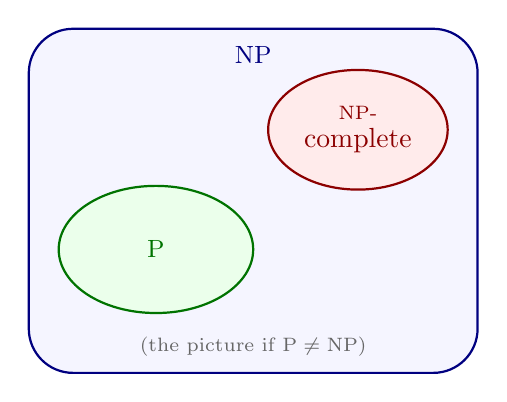
\begin{tikzpicture}[scale=0.95]
  % Assuming P != NP world
  \draw[rounded corners=16pt, fill=blue!4, draw=blue!50!black, thick]
    (-3.0,-2.3) rectangle (3.0,2.3);
  \node[blue!50!black] at (0,1.95) {\small $\mathrm{NP}$};
  % P blob
  \draw[fill=green!8, draw=green!45!black, thick] (-1.3,-0.65) ellipse (1.3 and 0.85);
  \node[green!45!black] at (-1.3,-0.65) {\small $\mathrm{P}$};
  % NP-complete blob (top right)
  \draw[fill=red!8, draw=red!55!black, thick] (1.4,0.95) ellipse (1.2 and 0.8);
  \node[red!55!black, align=center] at (1.4,0.95) {\scriptsize NP-\\[-2pt]complete};
  \node[font=\scriptsize, text=gray!80!black] at (0,-1.95) {(the picture if $\mathrm{P}\ne\mathrm{NP}$)};
\end{tikzpicture}
\caption{The conjectured complexity structure. $\mathrm{P}$ sits inside $\mathrm{NP}$. The
NP-complete problems are the ``hardest'' members of $\mathrm{NP}$, pushed up
against the far wall. If $\mathrm{P}=\mathrm{NP}$, the whole picture collapses to
a single blob.}
\label{ch33:landscape}
\end{figure}

\section{Reductions: ``no harder than''}

We now need a way to \emph{compare} the difficulty of two problems without
solving either of them. The tool is a \emph{reduction}: a way of transforming one
problem into another so cleanly that a solver for the second hands you a solver
for the first.

\begin{intuitionbox}
A reduction is a translator. Suppose you face problem $A$ but you only own a
machine that solves problem $B$. If you can rephrase any instance of $A$ as an
equivalent instance of $B$ -- preserving the yes/no answer -- then you can solve
$A$ by translating and feeding it to your $B$-machine. The translation says: ``$A$
is \emph{no harder than} $B$, give or take the cost of translating.'' If the
translation itself is cheap (polynomial), then $A$ piggybacks on $B$ entirely.
\end{intuitionbox}

\begin{formalbox}
\textbf{Polynomial-time reduction.} A language $A$ \emph{reduces in polynomial
time} to a language $B$, written $A \le_{\mathrm{P}} B$, if there is a
polynomial-time computable function $f$ (the reduction) such that for every input
$x$:
\[
  x \in A \quad\Longleftrightarrow\quad f(x) \in B.
\]
That is, $f$ maps \textsc{yes}-instances of $A$ to \textsc{yes}-instances of $B$,
and \textsc{no} to \textsc{no}, and $f$ runs in polynomial time.
\end{formalbox}

The direction of the inequality trips everyone up at first, so let us nail it
down with the two facts that make reductions useful.

\begin{lemma}[Reductions transfer easiness and hardness]
\label{ch33:transfer}
Suppose $A \le_{\mathrm{P}} B$. Then:
\begin{enumerate}
  \item If $B \in \mathrm{P}$, then $A \in \mathrm{P}$. \quad(Easiness flows
        \emph{backward}: if the target is easy, so is the source.)
  \item If $A \notin \mathrm{P}$, then $B \notin \mathrm{P}$. \quad(Hardness flows
        \emph{forward}: if the source is hard, so is the target.)
\end{enumerate}
\end{lemma}

\begin{proof}
For (1): to decide whether $x \in A$, compute $f(x)$ in polynomial time, then run
the polynomial-time decider for $B$ on $f(x)$. Because $x\in A \iff f(x)\in B$,
this answers correctly. The total time is polynomial (translate) plus polynomial
(decide $B$), composed on an input that has grown only polynomially -- still
polynomial. So $A\in\mathrm{P}$.

Statement (2) is just the contrapositive of (1): if $A\notin\mathrm{P}$ then $B$
cannot be in $\mathrm{P}$, for if it were, (1) would force $A\in\mathrm{P}$.
\end{proof}

\begin{trapbox}
Reductions point ``uphill toward hardness.'' To prove a \emph{new} problem $B$ is
hard, you reduce a \emph{known-hard} problem $A$ \emph{into} $B$: $A \le_{\mathrm
P} B$. Students constantly do it backward -- reducing the new problem into a known
one -- which proves the new problem is \emph{easy}, the opposite of what they
wanted. Memorize the slogan: \emph{to show $B$ is hard, turn a hard $A$ into
$B$.} The hard problem you already trust is the \emph{source}; the new suspect is
the \emph{target}.
\end{trapbox}

\section{NP-completeness: the hardest problems in NP}

We can now state the central definition. An NP-complete problem is a problem in
$\mathrm{NP}$ that is \emph{at least as hard as every other problem in
$\mathrm{NP}$} -- everything reduces to it.

\begin{formalbox}
\textbf{NP-completeness.} A language $L$ is \emph{NP-complete} if:
\begin{enumerate}
  \item $L \in \mathrm{NP}$ (it is checkable), and
  \item for \emph{every} language $A \in \mathrm{NP}$, we have $A
        \le_{\mathrm{P}} L$ (everything in $\mathrm{NP}$ reduces to $L$).
\end{enumerate}
A problem satisfying only condition (2) -- hard for all of $\mathrm{NP}$, but not
necessarily in $\mathrm{NP}$ itself -- is called \emph{NP-hard}.
\end{formalbox}

This is an astonishing kind of object. Condition (2) says $L$ is a universal
target: \emph{any} checkable problem in the universe can be encoded as an instance
of $L$. If you had a polynomial algorithm for one NP-complete problem, you would
have one for \emph{all} of $\mathrm{NP}$, and $\mathrm{P}$ would equal
$\mathrm{NP}$.

\begin{focusbox}
The central consequence:
\[
  \text{If any NP-complete problem is in } \mathrm{P},
  \text{ then } \mathrm{P}=\mathrm{NP}.
\]
The NP-complete problems live or die together. Crack one and you crack them all;
conversely, the widespread failure to crack \emph{any} of them, despite decades of
effort by brilliant people, is the strongest practical evidence that
$\mathrm{P}\ne\mathrm{NP}$.
\end{focusbox}

But condition (2) quantifies over \emph{every} problem in $\mathrm{NP}$ -- an
infinite, open-ended collection. How could you ever prove such a thing for even a
single $L$? Cook and Levin proved that anchor theorem directly for \textsc{SAT}
in 1971, and once that single problem was established, single reductions sufficed
for every problem after it.

\subsection{The first domino: Cook--Levin}

\begin{theorem}[Cook--Levin, 1971]
\label{ch33:cook-levin}
The problem \textsc{SAT} -- ``is this Boolean formula satisfiable?'' -- is
NP-complete.
\end{theorem}

We will not grind through the full proof (it is technical, and CLRS \S34.3 does it
carefully), but the core construction is direct and illuminating. A
\textsc{SAT} instance is a logical formula built from Boolean variables
$x_1,\dots,x_n$ using AND ($\wedge$), OR ($\vee$), and NOT ($\neg$). The formula
is \emph{satisfiable} if there is some assignment of \textsc{true}/\textsc{false}
to the variables that makes the whole thing evaluate to \textsc{true}.

Why is \emph{every} NP problem reducible to \textsc{SAT}? Because a Boolean
formula is, in a deep sense, the most general thing a computer \emph{is}. Take any
problem $A\in\mathrm{NP}$ with its polynomial-time verifier $V$. The verifier is
ultimately a circuit of logic gates churning through the input $x$ and a guessed
certificate $y$. Cook's reduction builds, from $V$ and $x$, a giant Boolean
formula whose variables encode ``the certificate $y$'' and ``the entire step-by-
step computation of $V$ on $(x,y)$.'' Clauses of the formula enforce that the
computation is \emph{legal} (each step follows the verifier's rules) and that it
\emph{accepts}. The formula is satisfiable precisely when there exists a
certificate $y$ that makes $V$ accept -- i.e.\ precisely when $x\in A$. Because
$V$ runs in polynomial time, the formula has polynomial size, so the translation
is polynomial.

\begin{intuitionbox}
Think of \textsc{SAT} as the assembly language of $\mathrm{NP}$. Any verification
procedure, no matter how it is described, can be ``compiled down'' into a Boolean
formula that simulates it. Satisfiability of that formula \emph{is} the existence
of a valid certificate. That is why \textsc{SAT} can stand in for every other
problem in $\mathrm{NP}$ at once: logic is universal enough to mimic any
computation.
\end{intuitionbox}

\subsection{The chain reaction: how to prove a problem NP-complete}

Cook--Levin gives us our \emph{first} NP-complete problem the hard way -- by
arguing about all of $\mathrm{NP}$ directly. Every problem after that is proved
NP-complete the \emph{easy} way, by a single reduction from a problem we already
trust. Here is the recipe, and you will use it for the rest of the chapter.

\begin{focusbox}
\textbf{To prove a new problem $L$ is NP-complete:}
\begin{enumerate}
  \item Show $L \in \mathrm{NP}$: describe a short certificate and a
        polynomial-time check for it.
  \item Pick a problem $K$ \emph{already known} to be NP-complete.
  \item Give a polynomial-time reduction $K \le_{\mathrm{P}} L$: a translation
        turning any instance of $K$ into an instance of $L$ with the
        \emph{same} yes/no answer.
\end{enumerate}
Step 3 is the creative one. The translation only \emph{transfers} hardness; it
relies on $K$ being a previously established NP-complete problem.
\end{focusbox}

Why does this work? Because reductions \emph{compose}. If $K$ is NP-complete then
every $A\in\mathrm{NP}$ satisfies $A\le_{\mathrm P}K$. If we also show $K\le_{
\mathrm P}L$, then for every $A\in\mathrm{NP}$ we can chain the translations,
$A\le_{\mathrm P}K\le_{\mathrm P}L$, so $A\le_{\mathrm P}L$. Combined with $L\in
\mathrm{NP}$, that is exactly the definition of NP-complete. One new reduction
inherits the entire infinite cone of hardness below $K$.

\begin{lemma}[Reductions compose]
\label{ch33:compose}
If $A\le_{\mathrm P}B$ and $B\le_{\mathrm P}C$, then $A\le_{\mathrm P}C$.
\end{lemma}
\begin{proof}
Let $f$ reduce $A$ to $B$ and $g$ reduce $B$ to $C$. Then $x\in A \iff f(x)\in B
\iff g(f(x))\in C$, so $g\circ f$ reduces $A$ to $C$. Both $f$ and $g$ are
polynomial-time and $f(x)$ has polynomial length, so computing $g(f(x))$ is
polynomial-time. Hence $g\circ f$ is a valid polynomial-time reduction.
\end{proof}

The rest of the chapter walks the historical tree of reductions. Each arrow below
is a single proof we will either sketch or do in full.

\begin{figure}[h]
\centering
\begin{tikzpicture}[
  node distance=8mm,
  every node/.style={font=\small},
  prob/.style={draw, rounded corners=3pt, fill=red!6, draw=red!55!black,
               minimum height=7mm, inner sep=4pt},
  ar/.style={-{Stealth[length=2.2mm]}, thick, gray!60!black}]
  \node[prob] (sat) {\textsc{Sat}};
  \node[prob, below=of sat] (3sat) {\textsc{3-Sat}};
  \node[prob, below left=10mm and 6mm of 3sat] (clique) {\textsc{Clique}};
  \node[prob, below right=10mm and 6mm of 3sat] (subset) {\textsc{Subset-Sum}};
  \node[prob, below=12mm of clique] (vc) {\textsc{Vertex-Cover}};
  \node[prob, below=12mm of vc] (ham) {\textsc{Ham-Cycle}};
  \node[prob, below=10mm of ham] (tsp) {\textsc{Tsp}};
  \draw[ar] (sat) -- (3sat);
  \draw[ar] (3sat) -- (clique);
  \draw[ar] (3sat) -- (subset);
  \draw[ar] (clique) -- (vc);
  \draw[ar] (3sat.west) to[bend right=55] (ham.west);
  \draw[ar] (ham) -- (tsp);
\end{tikzpicture}
\caption{The reduction tree of this chapter. An arrow $X\to Y$ means ``we reduce
$X$ to $Y$,'' proving $Y$ NP-complete given that $X$ already is. Everything
ultimately roots at \textsc{Sat} via Cook--Levin.}
\label{ch33:reduction-tree}
\end{figure}

\section{From SAT to 3-SAT: taming the formula}

Our first reduction tidies \textsc{SAT} into a rigid, regular shape that is far
easier to build other reductions \emph{from}. A formula is in \emph{conjunctive
normal form} (CNF) if it is an AND of \emph{clauses}, each clause an OR of
\emph{literals}, where a literal is a variable or its negation. The problem
\textsc{3-SAT} restricts every clause to \emph{exactly three} literals:
\[
  (x_1 \vee \neg x_2 \vee x_3)\;\wedge\;(\neg x_1 \vee x_3 \vee x_4)\;\wedge\;
  (x_2 \vee \neg x_3 \vee \neg x_4).
\]
\textsc{3-SAT} asks whether such a 3-clause formula has a satisfying assignment.

\begin{theorem}
\label{ch33:3sat}
\textsc{3-SAT} is NP-complete.
\end{theorem}

\emph{Membership in $\mathrm{NP}$} is immediate: a satisfying assignment is a
certificate of length $n$, and evaluating the formula on it takes time linear in
the formula's size. \emph{Hardness} follows from $\textsc{SAT}\le_{\mathrm P}
\textsc{3-SAT}$. We convert an arbitrary formula into an equisatisfiable 3-CNF
formula in three mechanical steps: push negations inward, distribute to reach CNF,
then \emph{split long clauses} and \emph{pad short ones} so every clause has
exactly three literals.

The clever move is splitting a long clause. A clause like $(\ell_1 \vee \ell_2
\vee \ell_3 \vee \ell_4 \vee \ell_5)$ becomes a \emph{chain} of 3-clauses linked
by fresh ``connector'' variables $y_i$:
\[
  (\ell_1 \vee \ell_2 \vee y_1)\,\wedge\,
  (\neg y_1 \vee \ell_3 \vee y_2)\,\wedge\,
  (\neg y_2 \vee \ell_4 \vee \ell_5).
\]
\begin{figure}[h]
\centering
\begin{tikzpicture}[every node/.style={font=\footnotesize},
  cl/.style={draw, rounded corners=3pt, fill=blue!6, draw=blue!50!black,
             minimum height=8mm, inner sep=4pt},
  lnk/.style={-{Stealth[length=2mm]}, thick, quotientorange}]
  \node[cl] (c1) {$\ell_1 \vee \ell_2 \vee y_1$};
  \node[cl, right=14mm of c1] (c2) {$\neg y_1 \vee \ell_3 \vee y_2$};
  \node[cl, right=14mm of c2] (c3) {$\neg y_2 \vee \ell_4 \vee \ell_5$};
  \draw[lnk] (c1.east) -- node[above,font=\scriptsize]{$y_1$} (c2.west);
  \draw[lnk] (c2.east) -- node[above,font=\scriptsize]{$y_2$} (c3.west);
\end{tikzpicture}
\caption{Splitting the long clause $(\ell_1\vee\cdots\vee\ell_5)$ into a chain of
$3$-clauses. The fresh connector variables $y_1,y_2$ (orange) thread the clauses
together. If every $\ell_j$ is false, satisfying the first clause forces $y_1$
true, which forces $y_2$ true, which leaves the last clause unsatisfiable -- so
the chain is satisfiable exactly when some original $\ell_j$ is true.}
\label{ch33:chain-fig}
\end{figure}

Stare at this. If some original $\ell_j$ is true, you can set the connectors so
every new clause is satisfied. If \emph{every} $\ell_j$ is false, then to satisfy
the first clause you must set $y_1$ true, which forces (via $\neg y_1$) the second
to need $y_2$ true, which forces the last clause to fail -- there is no escape (Figure~\ref{ch33:chain-fig}). So
the chain is satisfiable exactly when the original long clause was. Short clauses
(one or two literals) are padded by duplicating a literal or adding dummy
variables. The whole conversion is polynomial in size, so $\textsc{SAT}\le_{
\mathrm P}\textsc{3-SAT}$. \qed

\begin{aestheticbox}
\textsc{3-SAT} is the universal starting point for NP-completeness proofs. Its structure -- a
fixed pile of variables, a fixed pile of three-literal clauses -- is just rigid
enough to ``wire up'' into other problems, like building a circuit out of a
uniform stock of components. Almost every hardness proof in this chapter and the
literature beyond starts from \textsc{3-SAT}, not raw \textsc{SAT}. When you want
to show your scheduling, layout, or game problem is hard, \textsc{3-SAT} is the
hammer you reach for first.
\end{aestheticbox}

\section{Clique: hardness becomes a graph}

Now we leave logic and enter graph theory -- and watch the hardness make the
jump. A \emph{clique} in an undirected graph is a set of vertices that are
\emph{all} pairwise adjacent: a little island of total connection. The problem
\textsc{Clique} asks: ``does graph $G$ contain a clique of size at least $k$?''

\begin{theorem}
\label{ch33:clique}
\textsc{Clique} is NP-complete.
\end{theorem}

\emph{In $\mathrm{NP}$:} the certificate is the set of $k$ vertices; checking that
all $\binom{k}{2}$ pairs are edges takes $O(k^2)$ time. For hardness we show
$\textsc{3-SAT}\le_{\mathrm P}\textsc{Clique}$, a beautiful reduction that turns
``can I satisfy this formula?'' into ``can I find a clique?''

\textbf{The construction.} Take a 3-CNF formula $\phi$ with $m$ clauses
$C_1,\dots,C_m$. Build a graph $G$ as follows. For each clause, create one vertex
per literal -- so $3m$ vertices total, arranged in $m$ groups of three. Now add an
edge between two literal-vertices $\ell$ (in clause $C_i$) and $\ell'$ (in clause
$C_j$) \emph{if and only if}:
\begin{itemize}
  \item they are in \emph{different} clauses ($i\ne j$), and
  \item they are \emph{not contradictory}, i.e.\ $\ell'$ is not the negation of
        $\ell$.
\end{itemize}
We deliberately put \emph{no} edges inside a clause. Set the target $k=m$, the
number of clauses.

\begin{figure}[h]
\centering
\begin{tikzpicture}[scale=1.0, every node/.style={font=\footnotesize},
  lit/.style={circle, draw=sourceblue!70!black, fill=sourceblue!8, inner sep=1.4pt, minimum size=6.5mm},
  pick/.style={circle, draw=trapred!80!black, fill=trapred!20, very thick, inner sep=1.4pt, minimum size=6.5mm}]
  % three clauses, columns
  \node[pick] (a1) at (0,2)   {$x_1$};
  \node[lit] (a2) at (0,1)   {$\neg x_2$};
  \node[lit] (a3) at (0,0)   {$\neg x_3$};
  \node[lit] (b1) at (3,2)   {$\neg x_1$};
  \node[pick] (b2) at (3,1)   {$x_2$};
  \node[lit] (b3) at (3,0)   {$x_3$};
  \node[lit] (c1) at (6,2)   {$x_1$};
  \node[pick] (c2) at (6,1)   {$x_2$};
  \node[lit] (c3) at (6,0)   {$x_3$};
  \node[font=\small\bfseries] at (0,2.8) {Clause $C_1$};
  \node[font=\small\bfseries] at (3,2.8) {Clause $C_2$};
  \node[font=\small\bfseries] at (6,2.8) {Clause $C_3$};
  % a few representative consistent cross-edges (not all, to stay readable)
  \draw[gray!45] (a1)--(b3);
  \draw[gray!45] (a1) to[bend left=24] (c1);
  \draw[gray!45] (a1) to[bend right=18] (c3);
  \draw[gray!45] (b2)--(c1); \draw[gray!45] (b3)--(c3);
  % The selected 3-clique
  \draw[trapred!80!black, very thick] (a1)--(b2);
  \draw[trapred!80!black, very thick] (b2)--(c2);
  \draw[trapred!80!black, very thick] (a1)--(c2);
\end{tikzpicture}
\caption{The \textsc{3-Sat}-to-\textsc{Clique} gadget for $\phi=(x_1\vee\neg x_2
\vee\neg x_3)\wedge(\neg x_1\vee x_2\vee x_3)\wedge(x_1\vee x_2\vee x_3)$. Edges
join non-contradictory literals in different clauses (only a few cross-edges are
drawn, to keep the picture readable). The highlighted red vertices $x_1 \in C_1$,
$x_2 \in C_2$, and $x_2 \in C_3$ form a $3$-clique corresponding to the
satisfying assignment $x_1=x_2=\textsc{true}$: exactly one true literal picked
per clause, mutually consistent across all clauses.}
\label{ch33:clique-gadget}
\end{figure}

\textbf{Why it works.} Suppose $\phi$ is satisfiable. Pick a satisfying
assignment, and in each clause select \emph{one} literal that the assignment makes
true. That gives $m$ literal-vertices, one per clause. Any two of them are in
different clauses (so eligible for an edge) and are both true under the same
assignment (so they cannot be a variable and its negation -- that would be
contradictory). Hence every pair is joined: these $m$ vertices form a clique of
size $m=k$.

Conversely, suppose $G$ has a clique of size $m$. Since there are no edges inside
a clause, the clique can include at most one vertex per clause -- and to reach
size $m$ it must include \emph{exactly} one from each. Because clique-vertices are
pairwise non-contradictory, we can consistently set every chosen literal to
\textsc{true} (no variable is asked to be both true and false). That assignment
makes one literal true in every clause, satisfying $\phi$.

So $\phi$ is satisfiable $\iff$ $G$ has an $m$-clique. The graph has $3m$ vertices
and is built in time polynomial in $|\phi|$. That completes $\textsc{3-SAT}\le_{
\mathrm P}\textsc{Clique}$, and \textsc{Clique} is NP-complete. \qed

\begin{intuitionbox}
The reduction is a \emph{translation of meaning}. ``Pick one true literal in each
clause'' became ``pick one vertex in each group.'' ``The picks must be logically
consistent'' became ``the picks must be pairwise connected.'' The geometry of the
graph is engineered so that the only large cliques are exactly the consistent
literal-selections. This pattern -- encode the constraints of one problem as the
adjacency structure of another -- drives every reduction in this chapter.
\end{intuitionbox}

\section{Vertex Cover: the same coin, flipped}

A \emph{vertex cover} of a graph is a set of vertices that \emph{touches every
edge}: every edge has at least one endpoint in the set. \textsc{Vertex-Cover}
asks: ``is there a vertex cover of size at most $k$?'' The direction has flipped
-- we want a \emph{small} cover, whereas \textsc{Clique} wanted a \emph{large}
clique.

\begin{theorem}
\label{ch33:vc}
\textsc{Vertex-Cover} is NP-complete.
\end{theorem}

\emph{In $\mathrm{NP}$:} the cover is the certificate; scan every edge and check
an endpoint is included, in $O(|E|)$ time. For hardness we reduce from
\textsc{Clique} -- and the reduction takes a single complementation step,
resting on one structural fact.

\begin{lemma}[Clique--cover duality]
\label{ch33:vc-duality}
Let $G$ have $n$ vertices, and let $\bar G$ be its \emph{complement} (same
vertices; an edge in $\bar G$ exactly where $G$ has none). Then $S$ is a clique of
size $k$ in $G$ if and only if $V \setminus S$ is a vertex cover of size $n-k$ in
$\bar G$.
\end{lemma}
\begin{proof}
$S$ is a clique in $G$ means every pair inside $S$ is an edge of $G$, i.e.\ no pair
inside $S$ is an edge of $\bar G$. So in $\bar G$, every edge has at least one
endpoint \emph{outside} $S$ -- that is, in $V\setminus S$. Thus $V\setminus S$
covers all edges of $\bar G$. Each step is an ``if and only if,'' so the
equivalence holds, and $|V\setminus S| = n-k$.
\end{proof}

\textbf{The reduction.} Given a \textsc{Clique} instance $(G,k)$, output the
\textsc{Vertex-Cover} instance $(\bar G,\,n-k)$. Computing the complement is
$O(n^2)$, certainly polynomial. By the lemma, $G$ has a $k$-clique $\iff$ $\bar G$
has a vertex cover of size $n-k$. So $\textsc{Clique}\le_{\mathrm P}\textsc{Vertex
-Cover}$, and \textsc{Vertex-Cover} is NP-complete. \qed

\begin{example}[A traced instance]
\label{ch33:vc-example}
Let $G$ be the 5-cycle on vertices $\{1,2,3,4,5\}$ with edges $12,23,34,45,51$,
and ask for a clique of size $k=2$. The complement $\bar G$ is the
\emph{other} 5-cycle, with edges $13,24,35,41,52$. The duality predicts a vertex
cover of size $n-k=5-2=3$ in $\bar G$. Indeed $\{1,2,3\}$ covers $\bar G$: edge
$13$ hits $1$, $24$ hits $2$, $35$ hits $3$, $41$ hits $1$, $52$ hits $2$. And
$\{4,5\}$ -- the complement of that cover -- is a clique in $G$ (the edge $45$).
The bookkeeping matches perfectly (Figure~\ref{ch33:vc-duality-fig}).
\end{example}

\begin{figure}[h]
\centering
\begin{tikzpicture}[scale=1.0, every node/.style={font=\footnotesize},
  v/.style={circle, draw, minimum size=6mm, inner sep=0pt},
  pick/.style={circle, draw, fill=structurepurple!25, draw=structurepurple,
               very thick, minimum size=6mm, inner sep=0pt}]
  % left: G = C5, clique {4,5}
  \begin{scope}[shift={(0,0)}]
    \node[v] (g1) at (90:1.4)  {$1$};
    \node[v] (g2) at (162:1.4) {$2$};
    \node[v] (g3) at (234:1.4) {$3$};
    \node[pick] (g4) at (306:1.4) {$4$};
    \node[pick] (g5) at (18:1.4)  {$5$};
    \draw (g1)--(g2)--(g3)--(g4)--(g5)--(g1);
    \draw[targetgreen, very thick] (g4)--(g5);
    \node at (0,-2.1) {$G=C_5$: clique $\{4,5\}$};
  \end{scope}
  % right: complement Gbar, cover {1,2,3}
  \begin{scope}[shift={(5.2,0)}]
    \node[pick] (h1) at (90:1.4)  {$1$};
    \node[pick] (h2) at (162:1.4) {$2$};
    \node[pick] (h3) at (234:1.4) {$3$};
    \node[v] (h4) at (306:1.4) {$4$};
    \node[v] (h5) at (18:1.4)  {$5$};
    \draw (h1)--(h3); \draw (h1)--(h4); \draw (h2)--(h4);
    \draw (h2)--(h5); \draw (h3)--(h5);
    \node at (0,-2.1) {$\bar G$: cover $\{1,2,3\}$};
  \end{scope}
\end{tikzpicture}
\caption{Clique--cover duality on the $5$-cycle of Example~\ref{ch33:vc-example}.
The size-$2$ clique $\{4,5\}$ in $G$ (left, green edge) is exactly the complement
of the size-$3$ vertex cover $\{1,2,3\}$ in $\bar G$ (right, shaded). Every edge
of $\bar G$ touches a shaded vertex; the two unshaded vertices $4,5$ are mutually
adjacent in $G$.}
\label{ch33:vc-duality-fig}
\end{figure}

\begin{trapbox}
Do not confuse \emph{small} and \emph{large}. \textsc{Clique} and
\textsc{Independent-Set} look for the \emph{largest} possible structure;
\textsc{Vertex-Cover} looks for the \emph{smallest}. The duality lemma shows they
are the same problem viewed from opposite ends -- maximizing a clique is
minimizing the leftover cover. When you read a hardness claim, always note
whether the target wants a max or a min; a careless flip turns a correct
reduction into nonsense.
\end{trapbox}

\subsection{The direct gadget reduction: 3-SAT to Vertex Cover}
\label{ch33:sec-3sat-to-vc}

While the complement reduction from \textsc{Clique} is delightfully short, there
is another reduction from \textsc{3-SAT} directly to \textsc{Vertex-Cover} that
every computer scientist should see once. It uses the classic technique of
\emph{component gadgets} wired together.

Given a 3-CNF formula $\phi$ with $n$ variables $x_1, \dots, x_n$ and $m$ clauses
$C_1, \dots, C_m$:
\begin{enumerate}
  \item \textbf{Variable gadgets}: For each variable $x_i$, construct an edge
        connecting two vertices labeled $x_i$ and $\neg x_i$. To cover this edge,
        any vertex cover must pick at least one of these two vertices ($n$
        vertices across all $n$ variables).
  \item \textbf{Clause gadgets}: For each clause $C_j = (\ell_{j1} \vee \ell_{j2}
        \vee \ell_{j3})$, construct a triangle of three vertices labeled by its
        literals. To cover the three edges of a triangle, any vertex cover must
        pick at least \emph{two} vertices ($2m$ vertices across all $m$
        clauses).
  \item \textbf{Wiring edges}: For each clause $C_j$, connect each of its three
        literal vertices to the corresponding literal vertex in its variable
        gadget.
\end{enumerate}
We ask: does the resulting graph $G$ have a vertex cover of size at most
$k = n + 2m$?

\begin{figure}[h]
\centering
\begin{tikzpicture}[scale=0.95, every node/.style={font=\footnotesize},
  var/.style={circle, draw=sourceblue!80!black, fill=sourceblue!10, minimum size=6.5mm, inner sep=0pt},
  clause/.style={circle, draw=targetgreen!80!black, fill=targetgreen!10, minimum size=6.5mm, inner sep=0pt},
  pick/.style={circle, draw=structurepurple!80!black, fill=structurepurple!25, very thick, minimum size=6.5mm, inner sep=0pt},
  wire/.style={dashed, thick, gray!70}
]
% Top lane: Variable gadgets
\node[font=\footnotesize\bfseries] at (-1.8, 3.0) {Variables:};

% x1 gadget
\node[pick] (x1) at (0, 3.4) {$x_1$};
\node[var] (nx1) at (0, 2.4) {$\neg x_1$};
\draw[thick] (x1) -- (nx1);

% x2 gadget
\node[pick] (x2) at (3, 3.4) {$x_2$};
\node[var] (nx2) at (3, 2.4) {$\neg x_2$};
\draw[thick] (x2) -- (nx2);

% x3 gadget
\node[var] (x3) at (6, 3.4) {$x_3$};
\node[pick] (nx3) at (6, 2.4) {$\neg x_3$};
\draw[thick] (x3) -- (nx3);

% Bottom lane: Clause gadget for C1 = (x1 v ~x2 v x3)
\node[font=\footnotesize\bfseries] at (-1.8, 0.5) {Clause $C_1$:};
\node[clause] (c_x1) at (1.2, 1.2) {$x_1$};
\node[pick] (c_nx2) at (3.0, -0.2) {$\neg x_2$};
\node[pick] (c_x3) at (4.8, 1.2) {$x_3$};

% Clause triangle edges
\draw[thick, targetgreen!80!black] (c_x1) -- (c_nx2) -- (c_x3) -- cycle;

% Wiring edges
\draw[wire] (c_x1) -- (x1);
\draw[wire] (c_nx2) -- (nx2);
\draw[wire] (c_x3) -- (x3);

% Labels for chosen vertices
\node[structurepurple!80!black, font=\scriptsize, above=2pt of x1] {true};
\node[structurepurple!80!black, font=\scriptsize, above=2pt of x2] {true};
\node[structurepurple!80!black, font=\scriptsize, below=2pt of nx3] {true};
\node[structurepurple!80!black, font=\scriptsize, below=3pt of c_nx2] {picked};
\node[structurepurple!80!black, font=\scriptsize, right=3pt of c_x3] {picked};
\end{tikzpicture}
\caption{The direct \textsc{3-Sat}-to-\textsc{Vertex-Cover} gadget reduction
for clause $C_1 = (x_1 \vee \neg x_2 \vee x_3)$. Variable gadgets (top) force
at least $1$ vertex per variable into any cover. Clause triangles (bottom) force
at least $2$ vertices per clause. Setting $x_1=\textsc{true}$, $x_2=\textsc{true}$,
$x_3=\textsc{false}$ satisfies $C_1$ through literal $x_1$; its dashed wiring
edge is covered by $x_1$ in the variable gadget, allowing the remaining two
clause vertices ($\neg x_2$ and $x_3$) to cover the triangle and all remaining
wires. Total cover size is exactly $k = n + 2m = 3 + 2(1) = 5$.}
\label{ch33:fig-3sat-vc-gadget}
\end{figure}

\begin{intuitionbox}
Notice the arithmetic: any vertex cover requires at least $n$ vertices to cover
the $n$ variable edges, and at least $2m$ vertices to cover the $m$ disjoint
clause triangles. To reach the budget $k = n + 2m$, the cover must take
\emph{exactly} one vertex per variable (encoding a consistent assignment) and
\emph{exactly} two vertices per clause triangle. The third vertex in each clause
triangle is left uncovered from below, so its dashed wiring edge \emph{must} be
covered from above by the chosen variable vertex! Thus every clause contains at
least one true literal.
\end{intuitionbox}

\section{Hamiltonian Cycle and the Traveling Salesman}

We met \textsc{Ham-Cycle} in Example~\ref{ch33:ham-in-np}: does a graph have a
closed tour visiting every vertex exactly once? It too is NP-complete; the
reduction (from \textsc{3-SAT}, via intricate ``gadgets'' that simulate variables
and clauses with little chains of vertices) is genuinely involved, so we will
state the result and instead spend our energy on its famous corollary.

\begin{theorem}
\label{ch33:ham}
\textsc{Ham-Cycle} is NP-complete.
\end{theorem}

The reduction's flavor is worth a sentence. One builds, for each variable, a long
two-way ``ladder'' that any Hamiltonian cycle must traverse either left-to-right
or right-to-left -- and that binary choice \emph{is} the variable's truth value.
Small clause-gadgets are wired into the ladders so that the cycle can complete its
tour if and only if every clause is satisfied by the chosen traversal directions.
The variables' two-way streets encode \textsc{true}/\textsc{false}; the clauses
act as gates that the tour can only pass through when satisfied. It is fiddly, but
it is the same idea as the \textsc{Clique} reduction -- encode logic as structure
-- scaled up.

\subsection{TSP: putting numbers on the edges}

Now for one of the most famous problems in all of computing. The \emph{traveling
salesman} must visit a set of cities and return home, and wants the
\emph{cheapest} possible round trip. As a decision problem, \textsc{TSP} asks:
given cities, pairwise distances, and a budget $B$, is there a tour visiting all
cities exactly once with total length at most $B$?

\begin{theorem}
\label{ch33:tsp}
\textsc{TSP} is NP-complete.
\end{theorem}

\emph{In $\mathrm{NP}$:} a tour is the certificate; sum its edge lengths and
compare to $B$ in $O(n)$ time. For hardness we reduce from \textsc{Ham-Cycle},
and this reduction is short and elegant -- a perfect closing example because it
shows hardness leaping from a purely structural problem to a numeric optimization
one.

\textbf{The reduction.} Given a graph $G$ on $n$ vertices, build a \textsc{TSP}
instance whose ``cities'' are the vertices of $G$, with the \emph{complete}
distance matrix
\[
  d(u,v) =
  \begin{cases}
    1 & \text{if } (u,v) \text{ is an edge of } G,\\
    2 & \text{if } (u,v) \text{ is \emph{not} an edge of } G,
  \end{cases}
\]
and set the budget $B = n$. The matrix is built in $O(n^2)$ time.

\begin{figure}[h]
\centering
\begin{tikzpicture}[scale=1.0, every node/.style={font=\footnotesize},
  c/.style={circle, draw, fill=blue!8, minimum size=6mm, inner sep=0pt}]
  \node[c] (a) at (90:1.5)  {$a$};
  \node[c] (b) at (18:1.5)  {$b$};
  \node[c] (cc) at (-54:1.5) {$c$};
  \node[c] (d) at (-126:1.5) {$d$};
  \node[c] (e) at (162:1.5)  {$e$};
  % real edges of G (cost 1) -- a 5-cycle, which is a Ham cycle
  \draw[targetgreen, very thick] (a)--(b) node[midway,above right]{$1$};
  \draw[targetgreen, very thick] (b)--(cc) node[midway,right]{$1$};
  \draw[targetgreen, very thick] (cc)--(d) node[midway,below]{$1$};
  \draw[targetgreen, very thick] (d)--(e) node[midway,left]{$1$};
  \draw[targetgreen, very thick] (e)--(a) node[midway,above left]{$1$};
  % a non-edge (cost 2), drawn dashed across
  \draw[trapred, dashed] (a)--(cc) node[midway,sloped,above]{$2$};
\end{tikzpicture}
\caption{The \textsc{Ham-Cycle}-to-\textsc{TSP} reduction. Real edges of $G$ get
distance $1$ (solid green); every non-edge gets distance $2$ (dashed red, one
shown). A tour of $n=5$ cities uses $5$ edges, so the only way to hit the budget
$B=5$ is to ride entirely on cost-$1$ edges -- that is, on a Hamiltonian cycle of
$G$. A single cost-$2$ edge would push the total to $6>B$.}
\label{ch33:tsp-fig}
\end{figure}

\textbf{Why it works} (Figure~\ref{ch33:tsp-fig})\textbf{.} A \textsc{TSP} tour
visits all $n$ cities and uses exactly
$n$ edges (it is a cycle). Each edge costs $1$ or $2$, so the cheapest conceivable
tour costs $n$ -- achieved \emph{only} if every single edge it uses costs $1$,
i.e.\ every consecutive pair of cities is a genuine edge of $G$. But a tour
visiting every vertex once using only real edges of $G$ is precisely a
Hamiltonian cycle! So:
\[
  G \text{ has a Hamiltonian cycle}
  \iff
  \text{there is a tour of length} \le n=B.
\]
If $G$ has a Hamiltonian cycle, follow it: cost exactly $n\le B$. If the
\textsc{TSP} instance has a tour of length $\le n$, every edge it uses must cost
$1$ (any cost-$2$ edge would push the total above $n$), so the tour rides only on
edges of $G$ -- a Hamiltonian cycle. Hence $\textsc{Ham-Cycle}\le_{\mathrm P}
\textsc{TSP}$, and \textsc{TSP} is NP-complete. \qed

\begin{aestheticbox}
\textsc{TSP} is the public face of NP-completeness: delivery routing, circuit-
board drilling, DNA sequencing, and telescope scheduling all take this form. Its
NP-completeness does \emph{not} mean it is hopeless -- real solvers route
thousands of cities daily. It means there is (almost certainly) no algorithm that
is fast \emph{and} exact \emph{and} general all at once. In practice you give up
one of those: settle for ``almost optimal'' (approximation, Chapter 34), or
exploit special structure (cities in the plane behave better), or let a solver
grind on a particular instance. Proving a problem NP-complete does not mean
giving up on solving it in practice; it tells you to stop searching for an exact
worst-case polynomial algorithm on arbitrary inputs and instead adopt one of
those strategies.
\end{aestheticbox}

\section{Subset-Sum: when small numbers hide big inputs}

We close the gallery with a problem that looks utterly unlike a graph and teaches
the subtlest lesson of the chapter. \textsc{Subset-Sum}: given a multiset of
positive integers $\{a_1,\dots,a_n\}$ and a target $t$, is there a subset that
sums \emph{exactly} to $t$?

\begin{theorem}
\label{ch33:subset-sum}
\textsc{Subset-Sum} is NP-complete.
\end{theorem}

\emph{In $\mathrm{NP}$:} the certificate is the subset; add up its elements and
compare to $t$, in $O(n)$ additions. Hardness follows from $\textsc{3-SAT}\le_{
\mathrm P}\textsc{Subset-Sum}$ via a clever number-encoding: each variable and
each clause gets its own ``decimal column,'' and we craft numbers so that hitting
the target requires choosing one truth value per variable while filling every
clause's column to a fixed amount -- forcing each clause to be satisfied. The
arithmetic of carries is rigged to never interfere across columns. (CLRS \S34.5.5
builds it digit by digit; the construction is a small marvel and well worth
reading once you trust the pattern.)

\begin{trapbox}
``But \textsc{Subset-Sum} has an easy dynamic program!'' -- a fair objection, and
exactly the trap this section exists to spring. In Chapter 15 you built a table
of size $n\times t$ and filled it in $O(nt)$ time. So is \textsc{Subset-Sum} in
$\mathrm{P}$? \emph{No.} The catch is that $t$ is a \emph{number}, but the input
\emph{size} is the number of \emph{bits} needed to write everything down, and $t$
takes only about $\log_2 t$ bits. So $O(nt)$ is $O(n\cdot 2^{\log_2 t})$ --
\emph{exponential} in the input length (Figure~\ref{ch33:pseudo-fig}). Writing
$t$ in binary is cheap; counting up to $t$ is not.
\end{trapbox}

Here the warning from the first section becomes concrete: input size
counts \emph{symbols}, not magnitudes. An algorithm whose running time is
polynomial in the numeric \emph{value} of the inputs (here, in $t$) -- but
exponential in their bit-length -- is called \emph{pseudo-polynomial}. It can be
genuinely useful when the numbers are small, but it does \emph{not} place the
problem in $\mathrm{P}$, and it does not threaten $\mathrm{P}\ne\mathrm{NP}$.

\begin{figure}[h]
\centering
\begin{tikzpicture}[every node/.style={font=\footnotesize}]
  % a wide bar = value t, a tiny bar = bits of t
  \draw[fill=trapred!18, draw=trapred] (0,0.6) rectangle (9,1.2);
  \node at (4.5,0.9) {value $t \approx 10^{18}$: the table has this many columns};
  \draw[fill=sourceblue!22, draw=sourceblue] (0,-0.2) rectangle (0.62,0.4);
  \node[anchor=west] at (0.8,0.1) {bits of $t$ (about $\log_2 t \approx 60$): the input length};
\end{tikzpicture}
\caption{Why the $O(nt)$ table is not polynomial. The work is proportional to the
\emph{value} $t$ (long red bar), but the input is only the \emph{bits} of $t$
(short blue bar), about $\log_2 t$ of them. Each extra bit roughly \emph{doubles}
$t$, so the running time is exponential in the input length even though it looks
linear in $t$.}
\label{ch33:pseudo-fig}
\end{figure}

\begin{formalbox}
\textbf{Pseudo-polynomial vs.\ polynomial.} An algorithm is
\emph{polynomial-time} if its running time is bounded by a polynomial in the
input \emph{length} (the number of bits/symbols). It is merely
\emph{pseudo-polynomial} if its running time is polynomial in the input length
\emph{and} in the largest numeric value appearing in the input. The
$O(nt)$ table for \textsc{Subset-Sum} is pseudo-polynomial: polynomial in $n$ and
in the \emph{value} $t$, but exponential in the \emph{bits} of $t$.
\end{formalbox}

\begin{walkbox}
On your next walk, consider this question: why does the bit-length convention feel right?
Imagine an ``algorithm'' that solves a problem by counting from $1$ up to the
input number $N$. Its running time is $O(N)$ -- linear in the value, surely
``fast''? But to make $N$ a hundred times bigger you add only about seven bits to
the input, while the running time grows a hundredfold. Any sensible measure of
efficiency must punish that. Charging by bits, not by magnitude, is what makes
``polynomial time'' line up with our gut sense of ``scales gracefully.''
\end{walkbox}

\section{A worked reduction, end to end}

Reductions are a skill, and skills come from doing. Let us run one all the way
through on a tiny instance, gluing together the pieces above to feel the hardness
travel. We start from a concrete \textsc{3-SAT} formula and reduce it to
\textsc{Clique}, then read the answer back.

\begin{labbox}
Take the formula
\[
  \phi = (x_1 \vee x_2 \vee \neg x_3)\;\wedge\;
         (\neg x_1 \vee \neg x_2 \vee x_3)\;\wedge\;
         (x_1 \vee \neg x_2 \vee x_3).
\]
\textbf{Step 1 -- build the graph.} It has $3$ clauses, so $9$ vertices in $3$
groups:
\[
  C_1: \{x_1, x_2, \neg x_3\}, \quad
  C_2: \{\neg x_1, \neg x_2, x_3\}, \quad
  C_3: \{x_1, \neg x_2, x_3\}.
\]
Connect every pair from \emph{different} groups unless they contradict (one is the
negation of the other). For instance $x_1\in C_1$ connects to $\neg x_2, x_3\in
C_2$ but \emph{not} to $\neg x_1\in C_2$.

\textbf{Step 2 -- hunt for a $3$-clique.} Try the trio
$\{x_1(C_1),\, x_3(C_2),\, x_1(C_3)\}$. Different groups? Yes. Pairwise
non-contradictory? $x_1$ vs.\ $x_3$: fine. $x_1$ vs.\ $x_1$: same literal, not a
contradiction, fine. $x_3$ vs.\ $x_1$: fine. All three pairs are edges -- a
$3$-clique!

\textbf{Step 3 -- read off the assignment.} The clique used the literals $x_1,
x_3, x_1$, so set $x_1 = \textsc{true}$ and $x_3 = \textsc{true}$; $x_2$ is
unconstrained, say \textsc{false}. Check $\phi$: clause $1$ has $x_1$ true; clause
$2$ has $x_3$ true; clause $3$ has $x_1$ true. All satisfied. The clique we found
\emph{is} a satisfying assignment, exactly as the reduction promised.
\end{labbox}

\begin{algorithm}[H]
\caption{Generic NP-completeness proof template}
\KwIn{A decision problem $L$ you suspect is NP-complete}
\KwOut{A proof that $L$ is NP-complete (or a discovery that it is easy)}
\textbf{Step A (membership).} Exhibit a certificate $y$ for \textsc{yes}-instances
and a polynomial-time verifier $V(x,y)$\;
\If{no short, checkable certificate exists}{$L$ may be harder than $\mathrm{NP}$;
   stop and reconsider\;}
\textbf{Step B (choose a source).} Select a known NP-complete problem $K$ whose
structure resembles $L$ (often \textsc{3-Sat})\;
\textbf{Step C (reduce).} Design $f$ mapping each instance $w$ of $K$ to an
instance $f(w)$ of $L$\;
\textbf{Step D (correctness).} Prove $w\in K \iff f(w)\in L$ (both directions)\;
\textbf{Step E (efficiency).} Verify $f$ runs in time polynomial in $|w|$\;
\Return ``$L$ is NP-complete'' (Steps A and C--E together)\;
\end{algorithm}

\section{Demystifying the P vs.\ NP Discussion: A Plain-English Guide to Complexity Classes}
\label{ch33:demystifying-p-np}

For more than half a century, the discussion surrounding $\mathrm{P}$ versus $\mathrm{NP}$ has suffered from an unfortunate paradox: the central question is one of the most intuitive and philosophically captivating ideas in human thought, yet the surrounding terminology is notorious for confusing newcomers and experienced software engineers alike.

People routinely mix up $\mathrm{NP}$, $\mathrm{NP}$-complete, and $\mathrm{NP}$-hard. Many assume $\mathrm{NP}$ stands for ``not polynomial.'' Others wonder why finding the shortest traveling-salesman tour is treated differently from deciding whether a tour of length at most $B$ exists, or why integer factoring is the darling of public-key cryptography if it is not known to be $\mathrm{NP}$-complete.

Before exploring how engineers handle hardness in practice, let us step back from the gears of reduction gadgets and clarify the complete taxonomic map in plain English.

\subsection{Why the names are confusing (and how to never mix them up again)}

The vocabulary of complexity theory grew historically across logic, discrete mathematics, and early computer architecture. Table~\ref{ch33:tab-complexity-classes} and the narrative below contrast all six terms that arise in these discussions.

\begin{table}[htbp]
\centering
\small
\renewcommand{\arraystretch}{1.25}
\begin{tabular}{>{\bfseries}p{2.3cm} p{4.1cm} p{4.1cm} p{4.2cm}}
\toprule
Term & Plain-English Meaning & Intuitive Metaphor & Canonical Examples \\
\midrule
$\mathrm{P}$ &
Solvable from scratch in polynomial time $O(n^c)$. &
Calculating a driving route on a GPS unit. &
Shortest paths (Dijkstra), sorting, max flow, primality testing (AKS). \\

$\mathrm{NP}$ &
Verifiable in polynomial time when handed a hint. &
Checking whether a filled-in Sudoku grid is correct. &
All of $\mathrm{P}$, plus \textsc{3-Sat}, \textsc{Subset-Sum}, \textsc{Clique}, factoring. \\

$\mathrm{co\text{-}NP}$ &
Refutable in polynomial time with a single counterexample. &
Proving an argument is invalid by finding one flaw. &
\textsc{Tautology} (formula true on all inputs), \textsc{No-Hamilton-Cycle}. \\

$\mathrm{NP}$-Complete &
The hardest problems in $\mathrm{NP}$; every problem in $\mathrm{NP}$ reduces to them. &
A master key that can be shaped to open any door in a building. &
\textsc{3-Sat}, \textsc{Vertex-Cover}, \textsc{Clique}, \textsc{Ham-Cycle}, \textsc{Tsp} (decision). \\

$\mathrm{NP}$-Hard &
At least as hard as $\mathrm{NP}$-complete; not necessarily in $\mathrm{NP}$. &
A task so demanding it might not even have checkable answers. &
\textsc{Tsp} optimization (find minimum tour), the Halting Problem. \\

$\mathrm{NP}$-Intermediate &
Inside $\mathrm{NP}$, not in $\mathrm{P}$, yet likely not $\mathrm{NP}$-complete. &
A problem that resists fast solution without every $\mathrm{NP}$ problem reducing to it. &
Integer Factoring, Discrete Logarithm, Graph Isomorphism. \\
\bottomrule
\end{tabular}
\caption{The six primary terms in the $\mathrm{P}$ versus $\mathrm{NP}$ vocabulary, translated into plain English.}
\label{ch33:tab-complexity-classes}
\end{table}

Let us walk through each term carefully to understand why these boundaries exist:

\subsubsection{1. P: Easy to solve from scratch}
A problem lives in $\mathrm{P}$ if an ordinary deterministic computer can start from a cold input of size $n$ and calculate the exact answer within $O(n^c)$ clock ticks. You do not need divine inspiration, hints, or lucky guesses. Sorting a list, computing minimum spanning trees, finding shortest routes, and determining whether a number is prime (settled by Agrawal, Kayal, and Saxena in 2002 via the polynomial AKS primality test) all live comfortably in $\mathrm{P}$.

\subsubsection{2. NP: Easy to check when handed a hint}
The single most prevalent misunderstanding in computing is that $\mathrm{NP}$ means ``not polynomial.'' It does not. $\mathrm{NP}$ stands for \emph{nondeterministic polynomial time}, an antiquated name for a very clean concept: problems where verifying a proposed answer takes polynomial time.

Every problem in $\mathrm{P}$ is automatically in $\mathrm{NP}$: if you can solve something from scratch in polynomial time, you can verify a claimed answer by ignoring the certificate and solving it yourself. The mystery of $\mathrm{NP}$ comes from the problems that appear to be much harder to solve than to check:
\begin{itemize}
  \item Solving a 500-piece jigsaw puzzle might take you an entire weekend of trial and error; verifying a finished puzzle takes ten seconds of scanning the seams.
  \item Factoring a 600-digit number $N = p \times q$ defeats supercomputers; verifying that $p \times q = N$ requires one multiplication pass.
  \item Finding a formal proof for a mathematical conjecture can consume centuries; verifying that a formal proof in Lean or Coq contains no syntax or logic errors runs in seconds on a laptop.
\end{itemize}

\subsubsection{3. co-NP: Easy to disprove with a counterexample}
$\mathrm{co\text{-}NP}$ is the mirror universe of $\mathrm{NP}$.
Recall the asymmetry of $\mathrm{NP}$: for a \textsc{yes} instance, there is a short certificate that convinces you (the Hamiltonian tour, the satisfying assignment). But for a \textsc{no} instance (``this graph has no Hamiltonian cycle''), you seemingly have to rule out all factorial possibilities.

$\mathrm{co\text{-}NP}$ reverses this polarity. A problem is in $\mathrm{co\text{-}NP}$ if a \textsc{no} answer has a short, polynomial-time checkable certificate.

Consider the \textsc{Tautology} problem: given a Boolean formula $\phi$, is $\phi$ true for \emph{every possible truth assignment}?
\begin{itemize}
  \item If the answer is \textsc{no}, proving it is effortless: hand the verifier a single assignment that evaluates $\phi$ to \textsc{False}. That single counterexample is verified in linear time. Thus, \textsc{Tautology} is in $\mathrm{co\text{-}NP}$.
  \item If the answer is \textsc{yes}, how do you convince someone that \emph{no counterexample exists} anywhere among the $2^n$ possibilities? There is no known short witness.
\end{itemize}
Complexity theorists believe that $\mathrm{NP} \neq \mathrm{co\text{-}NP}$. If they were equal, every problem with a short proof of \textsc{yes} would also have a short proof of \textsc{no}.

\subsubsection{4. NP-Complete: The hardest problems in NP}
An $\mathrm{NP}$-complete problem is a problem inside $\mathrm{NP}$ with a universal translation property: \emph{every single problem in $\mathrm{NP}$ can be transformed into it in polynomial time}.

They are the hardest problems in $\mathrm{NP}$. As we have seen throughout this chapter, \textsc{3-Sat}, \textsc{Clique}, \textsc{Vertex-Cover}, \textsc{Hamiltonian-Cycle}, and \textsc{Subset-Sum} are all polynomial-time equivalent. If an engineer discovers a polynomial-time algorithm for any one of them, that single breakthrough would immediately solve every problem in $\mathrm{NP}$ in polynomial time, establishing $\mathrm{P} = \mathrm{NP}$.

\subsubsection{5. NP-Hard: At least as hard as NP-complete, maybe not even checkable}
This is the second great point of confusion. What is the difference between $\mathrm{NP}$-complete and $\mathrm{NP}$-hard?
\begin{itemize}
  \item To be \textbf{$\mathrm{NP}$-complete}, a problem must satisfy two conditions: it must be in $\mathrm{NP}$, and it must be $\mathrm{NP}$-hard.
  \item To be \textbf{$\mathrm{NP}$-hard}, a problem only needs to be at least as hard as $\mathrm{NP}$-complete problems. It does \emph{not} have to be in $\mathrm{NP}$, and it does \emph{not} even have to be a yes/no decision problem!
\end{itemize}

Consider two concrete examples of problems that are $\mathrm{NP}$-hard but \emph{not} in $\mathrm{NP}$:
\begin{enumerate}
  \item \textbf{The Optimization Version of Traveling Salesman (\textsc{Tsp}-Opt):} ``Given a list of cities and pairwise distances, find the tour of \emph{absolute minimum} total length.''
        Why is this not in $\mathrm{NP}$? Because if someone hands you a tour of length $412$, how do you verify in polynomial time that \emph{no tour of length $411$ exists}? To verify optimality, you would need to rule out all competing tours -- a $\mathrm{co\text{-}NP}$ task, not an $\mathrm{NP}$ task. Because it is not a decision problem with a polynomial certificate, it is not in $\mathrm{NP}$. But it is $\mathrm{NP}$-hard: if you could find the optimal tour instantly, you could immediately answer the yes/no decision version.
  \item \textbf{The Halting Problem ($\textsc{Halt}$):} As proved in Theorem~\ref{ch33:thm-halting}, deciding whether an arbitrary program halts is undecidable. Yet $\textsc{Halt}$ is $\mathrm{NP}$-hard! Any $\mathrm{NP}$ problem, such as \textsc{3-Sat}, reduces to $\textsc{Halt}$: given a formula $\phi$, construct a program that enumerates all assignments and halts if and only if it finds one that satisfies $\phi$. The program halts if and only if $\phi$ is satisfiable. Thus, $\textsc{Halt}$ is $\mathrm{NP}$-hard, even though it lies far beyond computable mathematics.
\end{enumerate}

\subsubsection{6. NP-Intermediate: The mysterious middle ground}
If $\mathrm{P} \neq \mathrm{NP}$, is every problem in $\mathrm{NP}$ either in $\mathrm{P}$ or $\mathrm{NP}$-complete?

In 1975, Richard Ladner proved that the answer is an emphatic \textbf{no}: if $\mathrm{P} \neq \mathrm{NP}$, there exists an infinite hierarchy of problems in $\mathrm{NP}$ that are provably not in $\mathrm{P}$, yet provably not $\mathrm{NP}$-complete. These problems are designated \textbf{$\mathrm{NP}$-intermediate}.

While Ladner's original proof used an artificial diagonal construction, real-world candidate problems appear to live precisely in this intermediate territory:
\begin{itemize}
  \item \textbf{Integer Factoring:} Given an integer $N$, find its prime factors. Factoring is in $\mathrm{NP}$ because checking that factors multiply to $N$ takes $O((\log N)^2)$ time. But Factoring is also in $\mathrm{co\text{-}NP}$: by the Fundamental Theorem of Arithmetic, prime factorizations are unique. A list of claimed prime factors along with primality certificates proves both what the factors are and that no other factors exist.
        Because Factoring lives in $\mathrm{NP} \cap \mathrm{co\text{-}NP}$, complexity theorists strongly believe it is \emph{not} $\mathrm{NP}$-complete. If Factoring were $\mathrm{NP}$-complete, it would imply $\mathrm{NP} = \mathrm{co\text{-}NP}$, an eventuality considered almost as unlikely as $\mathrm{P} = \mathrm{NP}$. This intermediate status is what makes RSA cryptography possible: factoring is hard enough that classical algorithms cannot break it in polynomial time, yet structured enough to support the algebraic symmetry of public-key encryption.
  \item \textbf{Graph Isomorphism:} Given two graphs $G_1$ and $G_2$, can the vertices of $G_1$ be relabeled to produce $G_2$? In 2015, L\'aszl\'o Babai proved that Graph Isomorphism can be solved in quasi-polynomial time ($2^{O((\log n)^c)}$). Because $2^{(\log n)^c}$ grows far slower than the $2^{\Omega(n)}$ time expected for $\mathrm{NP}$-complete problems, Graph Isomorphism is almost certainly intermediate rather than $\mathrm{NP}$-complete.
\end{itemize}

Figure~\ref{ch33:fig-p-vs-np-map} illustrates how these classes nest under the standard assumption that $\mathrm{P} \neq \mathrm{NP}$.

\begin{figure}[htbp]
\centering
\begin{tikzpicture}[font=\small, >=Latex, scale=0.91]
  % -------------------------------------------------------------
  % Panel (a): The Map of Complexity Classes (assuming P != NP)
  % -------------------------------------------------------------
  \begin{scope}[xshift=0cm, yshift=0cm]
    \node[anchor=west, font=\small\bfseries] at (-0.2, 4.55) {(a) Complexity Classes ($\mathrm{P} \neq \mathrm{NP}$)};

    % Outer NP-Hard boundary (above and around NP)
    \draw[dashed, thick, draw=trapred!70, fill=trapred!5, rounded corners=8pt]
      (-0.2, 2.25) rectangle (6.8, 3.85);
    \node[anchor=north west, font=\scriptsize\bfseries, text=trapred!90!black] at (0.0, 3.75) {$\mathrm{NP}$-Hard (Not necessarily in $\mathrm{NP}$)};
    \node[anchor=north west, font=\tiny, text=trapred!90!black, align=left] at (0.0, 3.37) {
      $\bullet$ \textsc{Tsp}-Optimization (find shortest tour)\\
      $\bullet$ Halting problem $\textsc{Halt}$ (undecidable)
    };

    % NP ellipse (left lobe)
    \draw[thick, draw=sourceblue!80, fill=sourceblue!10]
      (2.15, 0.7) ellipse (2.3cm and 1.35cm);
    \node[font=\footnotesize\bfseries, text=sourceblue!90!black] at (1.35, 1.52) {$\mathrm{NP}$};

    % co-NP ellipse (right lobe)
    \draw[thick, draw=quotientorange!80, fill=quotientorange!10]
      (4.45, 0.7) ellipse (2.3cm and 1.35cm);
    \node[font=\footnotesize\bfseries, text=quotientorange!90!black] at (5.15, 1.52) {$\mathrm{co\text{-}NP}$};

    % Intersection: NP \cap co-NP
    \begin{scope}
      \clip (2.15, 0.7) ellipse (2.3cm and 1.35cm);
      \draw[draw=none, fill=targetgreen!20] (4.45, 0.7) ellipse (2.3cm and 1.35cm);
    \end{scope}

    % P ellipse inside intersection
    \draw[thick, draw=targetgreen!90!black, fill=targetgreen!30]
      (3.3, 0.4) ellipse (1.05cm and 0.65cm);
    \node[font=\footnotesize\bfseries, text=targetgreen!95!black] at (3.3, 0.5) {$\mathrm{P}$};
    \node[font=\tiny, text=targetgreen!95!black] at (3.3, 0.15) {Dijkstra, AKS};

    % NP-Intermediate (Factoring) in (NP \cap co-NP) \ P
    \node[draw, fill=white, inner sep=1.5pt, rounded corners=2pt, font=\tiny, text=structurepurple!90!black] at (3.3, 1.38) {Factoring};

    % NP-Complete in left lobe
    \node[thick, draw=trapred!80, fill=trapred!20, rounded corners=3pt, inner sep=2.2pt, font=\tiny\bfseries, text=trapred!90!black, align=center] at (1.12, 0.82) {
      $\mathrm{NP}$-Complete\\[-1pt]
      {\normalfont\tiny \textsc{3-Sat}, \textsc{Clique}}
    };

    % co-NP-Complete in right lobe
    \node[thick, draw=quotientorange!90!black, fill=quotientorange!25, rounded corners=3pt, inner sep=2.2pt, font=\tiny\bfseries, text=quotientorange!95!black, align=center] at (5.48, 0.82) {
      $\mathrm{co\text{-}NP}$-Complete\\[-1pt]
      {\normalfont\tiny \textsc{Tautology}}
    };
  \end{scope}

  % -------------------------------------------------------------
  % Panel (b): Asymmetry of Generation vs. Verification
  % -------------------------------------------------------------
  \begin{scope}[xshift=7.8cm, yshift=0cm]
    \node[anchor=west, font=\small\bfseries] at (-0.2, 4.55) {(b) Discovery vs.\ Verification Asymmetry};

    % Box: Primes p and q
    \node[draw=sourceblue, fill=sourceblue!12, rounded corners=4pt, inner sep=4pt, align=center] (factors) at (1.1, 2.2) {
      \textbf{Prime Factors}\\
      \scriptsize $p = 61, \quad q = 53$\\
      \tiny (Secret witness / hint)
    };

    % Box: Product N
    \node[draw=quotientorange!80!black, fill=quotientorange!15, rounded corners=4pt, inner sep=4pt, align=center] (product) at (5.1, 2.2) {
      \textbf{Composite $N$}\\
      \scriptsize $N = p \times q = 3233$\\
      \tiny (Public problem instance)
    };

    % Multiplication arrow (Easy: P)
    \draw[->, very thick, targetgreen!80!black] (factors.north) to[out=35, in=145] node[above=2pt, font=\scriptsize\bfseries] {
      Multiply: $O((\log N)^2)$
    } node[below=2pt, font=\tiny, text=targetgreen!90!black] {\textbf{Tractable in P}} (product.north);

    % Factoring arrow (Hard: NP verification)
    \draw[->, very thick, trapred, dashed] (product.south) to[out=215, in=325] node[below=2pt, font=\scriptsize\bfseries] {
      Factor: Subexponential
    } node[above=2pt, font=\tiny, text=trapred!90!black, fill=white, inner sep=1.5pt] {\textbf{Hard to find, easy to check}} (factors.south);

    % Callout summary box at the bottom
    \node[draw=gray!50, fill=gray!6, rounded corners=4pt, inner sep=4pt, anchor=north, font=\tiny, align=left] at (3.1, 0.05) {
      \textbf{The Essence of NP:} Verification ($N \bmod p = 0$) takes $O((\log N)^2)$,\\
      while discovery from $N$ alone resists fast algorithms unless $\mathrm{P} = \mathrm{NP}$.
    };
  \end{scope}
\end{tikzpicture}
\caption{The taxonomy of computational complexity and the core asymmetry of verification. (a) Under the standard consensus that $\mathrm{P} \neq \mathrm{NP}$, the complexity classes cleanly separate: problems in $\mathrm{P}$ are solvable in polynomial time; $\mathrm{NP}$ contains problems whose solutions are verifiable in polynomial time; $\mathrm{co\text{-}NP}$ contains problems whose counterexamples are verifiable in polynomial time; $\mathrm{NP}$-Complete problems are the hardest problems in $\mathrm{NP}$; $\mathrm{NP}$-Intermediate problems like Factoring sit in $\mathrm{NP} \cap \mathrm{co\text{-}NP}$ outside $\mathrm{P}$ without being $\mathrm{NP}$-Complete; and $\mathrm{NP}$-Hard encompasses problems at least as hard as 3-SAT, including optimization and undecidable questions. (b) The asymmetric gulf between easy verification (in $\mathrm{P}$) and difficult search ($\mathrm{NP}$), exemplified by integer multiplication versus factoring.}
\label{ch33:fig-p-vs-np-map}
\end{figure}

\subsection{What is actually at stake: a day in a P = NP world}

Why does the $\mathrm{P}$ versus $\mathrm{NP}$ question capture imaginations far outside theoretical computer science? Because it asks whether creative discovery is fundamentally harder than clerical verification.

Consider what would happen if a researcher proved $\mathrm{P} = \mathrm{NP}$ by exhibiting a practical, low-degree polynomial-time algorithm for \textsc{3-Sat}:

\begin{itemize}
  \item \textbf{Public-key and symmetric cryptography break.} Modern digital security -- from HTTPS encryption and banking transactions to SSH keys and digital signatures -- rests entirely on the assumption that certain mathematical tasks are easy to perform in the forward direction but intractable to reverse without a secret key. Finding an AES-256 key that matches a given plaintext and ciphertext is an $\mathrm{NP}$ search problem: verifying a candidate key takes microseconds. If $\mathrm{P} = \mathrm{NP}$, cracking any symmetric or asymmetric cipher reduces to solving a polynomial-size SAT instance in minutes.
  \item \textbf{Mathematical theorem-proving is automated.} Is a famous mathematical conjecture of length $n$ provable in fewer than $M$ steps? An algorithm cannot easily guess the proof by brute force. But checking whether a candidate sequence of deductions constitutes a valid proof is a purely mechanical, polynomial-time verification pass. If $\mathrm{P} = \mathrm{NP}$, an algorithm could generate formal mathematical proofs of length $M$ as fast as a computer checks them. As Kurt G\"odel realized in his 1956 letter to John von Neumann, mathematical research itself would change fundamentally.
  \item \textbf{Scientific and industrial optimization becomes exact.} Designing a synthetic protein that folds to minimize free energy, routing hundreds of thousands of delivery vehicles with optimal fuel consumption, and floorplanning billions of transistors on a microprocessor without thermal bottlenecks are all $\mathrm{NP}$ search problems. A fast SAT solver would solve each of them to global mathematical optimality.
\end{itemize}

As computer scientist Scott Aaronson noted, if $\mathrm{P} = \mathrm{NP}$, then anyone who can appreciate a beautiful melody could compose like Mozart, and anyone who can follow a mathematical argument could discover breakthroughs like Gauss. The intuitive conviction that appreciating art or verifying a proof is vastly easier than creating it from nothing is our deepest daily evidence that $\mathrm{P} \neq \mathrm{NP}$.

\subsection{Why proving P $\neq$ NP is so hard: the three mathematical barriers}

If virtually every computer scientist believes $\mathrm{P} \neq \mathrm{NP}$, why has nobody managed to prove it in more than fifty years?

Consider the fundamental asymmetry of the challenge:
\begin{itemize}
  \item To prove $\mathrm{P} = \mathrm{NP}$, you only need to design \textbf{one} algorithm: an ingenious polynomial-time method for \textsc{3-Sat}.
  \item To prove $\mathrm{P} \neq \mathrm{NP}$, you must prove a sweeping impossibility theorem about \textbf{every conceivable algorithm that could ever be designed by any intelligence in the universe}.
\end{itemize}
You must prove that no algorithm -- no matter how unexpected its mechanics -- can ever solve \textsc{3-Sat} in polynomial time.

This is formidable because computer science is full of algorithms that perform surprising mathematical shortcuts. Naive matrix multiplication requires $8$ recursive multiplications of half-size blocks, leading to $O(n^3)$ time; Volker Strassen (1969) showed that an unexpected algebraic cancellation computes the product with only $7$ multiplications, dropping the exponent below $3$. Multiplying two degree-$n$ polynomials by convolution appears to require $O(n^2)$ coefficient operations; the Fast Fourier Transform (Cooley and Tukey, 1965) collapses the cost to $O(n \log n)$ by converting into the frequency domain. To prove $\mathrm{P} \neq \mathrm{NP}$, one must prove that \emph{no such algebraic shortcut exists} for any of the thousands of $\mathrm{NP}$-complete problems.

Whenever complexity theorists tried to prove lower bounds, their techniques repeatedly struck three fundamental structural barriers:

\begin{enumerate}
  \item \textbf{The Relativization Barrier (Baker, Gill, and Solovay, 1975):}
        Early impossibility results in computability (like the Halting Problem) relied on simulation and diagonalization. Baker, Gill, and Solovay proved that these techniques are ``relativizing''---they hold unchanged even if every machine is granted free, instantaneous access to an external black-box oracle $A$. They then constructed two oracles: an oracle $A$ where $\mathrm{P}^A = \mathrm{NP}^A$, and an oracle $B$ where $\mathrm{P}^B \neq \mathrm{NP}^B$. Therefore, any proof technique that relativizes is mathematically powerless to resolve $\mathrm{P}$ versus $\mathrm{NP}$.
  \item \textbf{The Natural Proofs Barrier (Razborov and Rudich, 1997):}
        Researchers next turned to circuit complexity, attempting to prove that small Boolean circuits cannot compute functions like \textsc{Clique}. Alexander Razborov and Steven Rudich demonstrated that almost all known circuit lower bound methods fall into a category they termed ``natural proofs'' (identifying a constructive combinatorial property common to random functions but rare in small circuits). They proved that if strong pseudorandom function generators exist (the foundation of modern cryptography), then no natural proof can ever separate $\mathrm{P}$ from $\mathrm{NP}$. In short: the very existence of cryptographic hardness prevents natural combinatorial arguments from proving that hardness!
  \item \textbf{The Algebrization Barrier (Aaronson and Wigderson, 2008):}
        In the 1990s, non-relativizing algebraic techniques successfully proved that $\mathrm{IP} = \mathrm{PSPACE}$. Scott Aaronson and Avi Wigderson proved that even when algebraic oracle extensions are permitted (``algebrization''), the barrier re-emerges: there exist algebraic oracles where the classes coincide and others where they separate.
\end{enumerate}

Any proof that separates $\mathrm{P}$ from $\mathrm{NP}$ must be simultaneously non-relativizing, non-natural, and non-algebrizing. It requires fundamentally new mathematical perspectives on computation, logic, and structure.

\section{What to do when your problem is NP-complete}

Suppose you have just proved -- or found in a textbook -- that the problem on your
desk is NP-complete. What now? You do \emph{not} give up, and you do \emph{not}
keep hunting for a fast exact general algorithm (that search is, by consensus,
doomed). Instead you bend one of the three rigid requirements ``fast, exact,
general.''

\begin{itemize}
  \item \textbf{Drop exactness -- approximate.} Accept a provably near-optimal
        answer. A good \textsc{Vertex-Cover} heuristic gets within a factor of $2$
        of optimal in linear time. This is the subject of the next chapter.
  \item \textbf{Drop generality -- exploit structure.} Real instances are not
        adversarial. \textsc{TSP} on points in the plane, \textsc{2-SAT} (clauses
        of size two -- actually in $\mathrm{P}$!), trees instead of general
        graphs: special cases routinely escape the hardness.
  \item \textbf{Drop speed in the worst case -- search smartly.} Branch-and-bound,
        SAT solvers, and integer-programming engines often crush real instances
        with thousands of variables, even though some adversarial input could in
        principle make them crawl.
  \item \textbf{Drop determinism -- randomize or use heuristics.} Simulated
        annealing, genetic algorithms, and local search give no guarantees but
        often deliver excellent answers fast.
\end{itemize}

\begin{focusbox}
The practical payoff of this whole chapter is a single reflex: \emph{before you
pour months into a perfect algorithm, check whether the problem is NP-complete.}
If it is, you have just saved yourself a hopeless search and redirected your
energy toward approximation, special-casing, or smart search -- the strategies
that actually ship.
\end{focusbox}

\subsection{The practical dividend of hardness}

The discovery of NP-completeness radically transformed the daily practice of
computer science:
\begin{itemize}
  \item \textbf{A shield against impossible engineering goals.} Before Karp and
        Cook, software engineers and researchers frequently spent years of
        futile effort attempting to invent polynomial-time algorithms for
        problems like Traveling Salesman or Boolean Satisfiability, assuming
        failure was merely their own lack of mathematical cleverness.
        NP-completeness gave engineers a definitive certificate: proving a
        problem is NP-complete shows that finding an exact polynomial
        algorithm is as hard as resolving the entire $\mathrm{P}$ versus
        $\mathrm{NP}$ question.
  \item \textbf{The SAT revolution in verification.} Cook's proof showed that
        Boolean logic is the universal substrate of computation. Decades later,
        engineers inverted this theoretical weapon into an industrial tool.
        Modern Conflict-Driven Clause Learning (CDCL) SAT and SMT solvers
        routinely compile microprocessor circuits, operating system drivers, and
        cryptographic protocols into millions of Boolean clauses, verifying
        hardware and software automatically.
  \item \textbf{The map of algorithmic unity.} NP-completeness showed that
        apparent differences between fields---graph theory, number theory,
        compiler register allocation, molecular biology, and operations
        research---are cosmetic. They all share an identical computational
        core.
\end{itemize}

\subsection{Coping with worst-case limits}

Despite its theoretical power, NP-completeness has practical boundaries:
\begin{itemize}
  \item \textbf{The tyranny of the worst case.} NP-completeness is an
        asymptotic, worst-case verdict. It asserts only that there exists
        \emph{some} pathological family of instances on which every algorithm
        stumbles. It says nothing about average-case instances or real-world
        distributions. In practice, industrial instances of \textsc{3-SAT},
        \textsc{TSP}, and \textsc{Knapsack} with thousands or millions of
        variables are routinely solved to optimality in seconds because
        real-world problem instances possess low treewidth, modularity, or
        geometric structure.
  \item \textbf{Polynomial reductions can hide large constants.} A
        reduction is declared efficient as long as its runtime is $O(n^c)$.
        A reduction that transforms an instance of size $n$ into an instance of
        size $n^{10}$ or requires $10^{10} n^2$ operations is theoretically in
        $\mathrm{P}$, but practically slow.
  \item \textbf{The unproven foundation.} Despite overwhelming consensus and a
        Clay Millennium Prize, $\mathrm{P} \ne \mathrm{NP}$ remains rigorously
        unproven. Decades of attempts to prove lower bounds using circuit complexity
        and diagonalization have run into deep structural barriers.
\end{itemize}

\begin{complexitybox}
A compact map of the chapter.
\begin{itemize}
  \item Undecidable: problems beyond algorithmic reach; the Halting Problem is uncomputable by Turing diagonalization ($D(\langle D \rangle)$), and Rice's theorem extends this to all non-trivial semantic properties.
  \item $\mathrm{P}$: solvable in time $O(n^c)$. ``Tractable.''
  \item $\mathrm{NP}$: \textsc{yes}-instances have a polynomial-size certificate
        checkable in polynomial time. Contains $\mathrm{P}$.
  \item $A\le_{\mathrm P}B$: a polynomial-time $f$ with $x\in A \iff f(x)\in B$.
        Hardness flows forward, easiness backward.
  \item NP-complete: in $\mathrm{NP}$ \emph{and} every $\mathrm{NP}$ problem
        reduces to it. One in $\mathrm{P}$ $\Rightarrow$ all of $\mathrm{NP}$ in
        $\mathrm{P}$.
  \item Cook--Levin: \textsc{Sat} is the first NP-complete problem. All others
        follow by single reductions:
        $\textsc{Sat}\!\le\!\textsc{3-Sat}\!\le\!\{\textsc{Clique},
        \textsc{Subset-Sum}\}$, $\textsc{Clique}\!\le\!\textsc{Vertex-Cover}$,
        $\textsc{3-Sat}\!\le\!\textsc{Ham-Cycle}\!\le\!\textsc{Tsp}$.
  \item Pseudo-polynomial: polynomial in input \emph{value}, not input
        \emph{length}. \textsc{Subset-Sum}'s $O(nt)$ table is this -- not a proof
        that the problem is in $\mathrm{P}$.
\end{itemize}
\end{complexitybox}

\section*{A closing thought}

NP-completeness is, oddly, a hopeful idea. It says that thousands of stubborn
problems across logic, graphs, scheduling, biology, and number theory are not a
ragged collection of unrelated nuisances -- they are all polynomial-time
translations of a single underlying search problem. Solve the salesman and you solve them all; fail on one and you
have likely failed on all. That unity is a gift. It means our ignorance is
organized. And it sharpens the greatest open question in the field to a single
crisp line -- $\mathrm{P}\overset{?}{=}\mathrm{NP}$ -- whose answer, whichever way
it falls, will be one of the deepest truths we ever learn about computation.

NP-completeness does not mean surrender. When an exact polynomial algorithm is out of reach, our goals adapt: we trade perfection for efficiency. In Chapter~34, we turn to approximation algorithms, designing algorithms that run in guaranteed polynomial time while provably bounding the distance between their solutions and the true optimum.

\section{Exercises}

\begin{exercise}[Certificates, warmup]
For each problem, state a short certificate for \textsc{yes}-instances and the
polynomial-time check that verifies it: (a) \textsc{Composite} (``is $N$ not
prime?''); (b) \textsc{Graph-3-Coloring} (``can $G$ be properly colored with $3$
colors?''); (c) \textsc{Subset-Sum}.
\end{exercise}

\begin{exercise}[The direction of reductions]
Your classmate proves $\textsc{New-Problem}\le_{\mathrm P}\textsc{3-SAT}$ and
concludes \textsc{New-Problem} is NP-complete. Explain precisely what is wrong,
and state what this reduction \emph{does} legitimately tell you about
\textsc{New-Problem}.
\end{exercise}

\begin{exercise}[Optimization to decision]
Describe carefully how a polynomial-time decider for the \emph{decision} version
of \textsc{TSP} (``is there a tour of length $\le B$?'') could be used to find the
exact length of the \emph{optimal} tour in polynomial time. (Hint: binary search
on $B$.) Why does this argument show the decision and optimization versions are
equally hard?
\end{exercise}

\begin{exercise}[Tracing 3-SAT to Clique]
Apply the \textsc{3-SAT}-to-\textsc{Clique} reduction to
$\phi = (x_1\vee x_2\vee x_3)\wedge(\neg x_1\vee\neg x_2\vee\neg x_3)$. Draw the
$6$-vertex graph, list its edges, find a $2$-clique, and read off a satisfying
assignment. Is there any $3$-clique? Explain why or why not.
\end{exercise}

\begin{exercise}[Clique--cover duality by hand]
Let $G$ be the complete graph $K_4$ (every pair of $4$ vertices adjacent). What is
the largest clique in $G$? Using Lemma~\ref{ch33:vc-duality}, what does that say
about the smallest vertex cover of $\bar G$? Verify directly by describing
$\bar G$.
\end{exercise}

\begin{exercise}[Independent sets]
An \emph{independent set} is a set of vertices with \emph{no} edges between them.
Prove that $S$ is an independent set of $G$ if and only if $V\setminus S$ is a
vertex cover of $G$. Conclude that \textsc{Independent-Set} is NP-complete by a
one-line reduction from \textsc{Vertex-Cover}.
\end{exercise}

\begin{exercise}[Hamiltonian path vs.\ cycle]
The \textsc{Ham-Path} problem asks for a path (not necessarily closed) visiting
every vertex exactly once. Give a polynomial-time reduction
$\textsc{Ham-Cycle}\le_{\mathrm P}\textsc{Ham-Path}$. (Hint: pick an edge of the
cycle to ``cut,'' or add a gadget vertex. Think about what turns a path into a
cycle.)
\end{exercise}

\begin{exercise}[Why exactly three?]
We reduced \textsc{Sat} to \textsc{3-SAT}. Suppose instead you restrict to
\textsc{2-SAT}: every clause has exactly two literals. It turns out \textsc{2-SAT}
is in $\mathrm{P}$. Where in the long-clause-splitting argument of
Theorem~\ref{ch33:3sat} would a ``split into $2$-clauses'' attempt break down?
(You need not solve \textsc{2-SAT}; just locate the obstruction.)
\end{exercise}

\begin{exercise}[Pseudo-polynomial, concretely]
The \textsc{Subset-Sum} table runs in $O(nt)$ time. (a) For $n=100$ numbers each
around $10^{18}$, estimate $t$ and the table size; is this practical? (b) Explain
in one sentence why this does not contradict NP-completeness. (c) Give an instance
family where the $O(nt)$ algorithm \emph{is} fast, and say what is special about
it.
\end{exercise}

\begin{exercise}[Build your own reduction -- challenge]
The \textsc{Set-Cover} problem: given a universe $U$ of elements, a collection of
subsets $S_1,\dots,S_m\subseteq U$, and a number $k$, can $k$ of the subsets cover
all of $U$? Prove \textsc{Set-Cover} is NP-complete by reducing
\textsc{Vertex-Cover} to it. (Hint: let the universe be the edges of the graph,
and let each vertex contribute the set of edges it touches.)
\end{exercise}

\begin{exercise}[A reduction that proves membership in P, not hardness -- challenge]
Consider \textsc{2-Coloring} (``can $G$ be properly $2$-colored?''). A student
tries to prove it NP-complete by reducing \textsc{3-Coloring} to it. Without doing
the reduction, argue why any such attempt must fail, assuming
$\mathrm{P}\ne\mathrm{NP}$. (Hint: \textsc{2-Coloring} is exactly the
bipartiteness test from Chapter 22 -- what complexity class is it in?)
\end{exercise}

\begin{exercise}[The halting contrarian by hand]
Recall the contrarian program $D$ from the proof of Theorem~\ref{ch33:thm-halting}.
Suppose a computer scientist claims to have implemented an analyzer \lstinline|Halts(P, x)| in $500$ lines of Python that handles all programs.
(a) Write out the exact $6$-line Python script for $D(\langle P \rangle)$ that uses this analyzer.
(b) Walk through the exact step-by-step evaluation of $D(\langle D \rangle)$, tracing the execution path if the analyzer returns \lstinline|True|, and tracing the path if it returns \lstinline|False|.
(c) Conclude why this contradiction implies that no static analyzer can ever be both sound (never miss an infinite loop) and complete (never falsely flag a terminating program) while always halting.
\end{exercise}

\begin{exercise}[Rice's Theorem in compiler optimization]
A compiler engineer attempts to build an optimization pass that automatically replaces any function computing the identity function $f(n) = n$ with a direct return instruction \lstinline|return n|.
(a) Define what it means for a property of programs to be \emph{semantic} versus \emph{syntactic}.
(b) Prove that ``computes the identity function'' is a non-trivial semantic property.
(c) Using Rice's Theorem (Theorem~\ref{ch33:thm-rice}), explain why no compiler optimization pass can ever identify \emph{all} functions that compute the identity function without either looping indefinitely on some inputs or using conservative heuristics that miss equivalent implementations.
\end{exercise}
